% Options for packages loaded elsewhere
\PassOptionsToPackage{unicode}{hyperref}
\PassOptionsToPackage{hyphens}{url}
\PassOptionsToPackage{dvipsnames,svgnames,x11names}{xcolor}
%
\documentclass[
  letterpaper,
  DIV=11,
  numbers=noendperiod]{scrartcl}

\usepackage{amsmath,amssymb}
\usepackage{iftex}
\ifPDFTeX
  \usepackage[T1]{fontenc}
  \usepackage[utf8]{inputenc}
  \usepackage{textcomp} % provide euro and other symbols
\else % if luatex or xetex
  \usepackage{unicode-math}
  \defaultfontfeatures{Scale=MatchLowercase}
  \defaultfontfeatures[\rmfamily]{Ligatures=TeX,Scale=1}
\fi
\usepackage{lmodern}
\ifPDFTeX\else  
    % xetex/luatex font selection
\fi
% Use upquote if available, for straight quotes in verbatim environments
\IfFileExists{upquote.sty}{\usepackage{upquote}}{}
\IfFileExists{microtype.sty}{% use microtype if available
  \usepackage[]{microtype}
  \UseMicrotypeSet[protrusion]{basicmath} % disable protrusion for tt fonts
}{}
\makeatletter
\@ifundefined{KOMAClassName}{% if non-KOMA class
  \IfFileExists{parskip.sty}{%
    \usepackage{parskip}
  }{% else
    \setlength{\parindent}{0pt}
    \setlength{\parskip}{6pt plus 2pt minus 1pt}}
}{% if KOMA class
  \KOMAoptions{parskip=half}}
\makeatother
\usepackage{xcolor}
\setlength{\emergencystretch}{3em} % prevent overfull lines
\setcounter{secnumdepth}{-\maxdimen} % remove section numbering
% Make \paragraph and \subparagraph free-standing
\ifx\paragraph\undefined\else
  \let\oldparagraph\paragraph
  \renewcommand{\paragraph}[1]{\oldparagraph{#1}\mbox{}}
\fi
\ifx\subparagraph\undefined\else
  \let\oldsubparagraph\subparagraph
  \renewcommand{\subparagraph}[1]{\oldsubparagraph{#1}\mbox{}}
\fi


\providecommand{\tightlist}{%
  \setlength{\itemsep}{0pt}\setlength{\parskip}{0pt}}\usepackage{longtable,booktabs,array}
\usepackage{calc} % for calculating minipage widths
% Correct order of tables after \paragraph or \subparagraph
\usepackage{etoolbox}
\makeatletter
\patchcmd\longtable{\par}{\if@noskipsec\mbox{}\fi\par}{}{}
\makeatother
% Allow footnotes in longtable head/foot
\IfFileExists{footnotehyper.sty}{\usepackage{footnotehyper}}{\usepackage{footnote}}
\makesavenoteenv{longtable}
\usepackage{graphicx}
\makeatletter
\def\maxwidth{\ifdim\Gin@nat@width>\linewidth\linewidth\else\Gin@nat@width\fi}
\def\maxheight{\ifdim\Gin@nat@height>\textheight\textheight\else\Gin@nat@height\fi}
\makeatother
% Scale images if necessary, so that they will not overflow the page
% margins by default, and it is still possible to overwrite the defaults
% using explicit options in \includegraphics[width, height, ...]{}
\setkeys{Gin}{width=\maxwidth,height=\maxheight,keepaspectratio}
% Set default figure placement to htbp
\makeatletter
\def\fps@figure{htbp}
\makeatother
% definitions for citeproc citations
\NewDocumentCommand\citeproctext{}{}
\NewDocumentCommand\citeproc{mm}{%
  \begingroup\def\citeproctext{#2}\cite{#1}\endgroup}
\makeatletter
 % allow citations to break across lines
 \let\@cite@ofmt\@firstofone
 % avoid brackets around text for \cite:
 \def\@biblabel#1{}
 \def\@cite#1#2{{#1\if@tempswa , #2\fi}}
\makeatother
\newlength{\cslhangindent}
\setlength{\cslhangindent}{1.5em}
\newlength{\csllabelwidth}
\setlength{\csllabelwidth}{3em}
\newenvironment{CSLReferences}[2] % #1 hanging-indent, #2 entry-spacing
 {\begin{list}{}{%
  \setlength{\itemindent}{0pt}
  \setlength{\leftmargin}{0pt}
  \setlength{\parsep}{0pt}
  % turn on hanging indent if param 1 is 1
  \ifodd #1
   \setlength{\leftmargin}{\cslhangindent}
   \setlength{\itemindent}{-1\cslhangindent}
  \fi
  % set entry spacing
  \setlength{\itemsep}{#2\baselineskip}}}
 {\end{list}}
\usepackage{calc}
\newcommand{\CSLBlock}[1]{\hfill\break\parbox[t]{\linewidth}{\strut\ignorespaces#1\strut}}
\newcommand{\CSLLeftMargin}[1]{\parbox[t]{\csllabelwidth}{\strut#1\strut}}
\newcommand{\CSLRightInline}[1]{\parbox[t]{\linewidth - \csllabelwidth}{\strut#1\strut}}
\newcommand{\CSLIndent}[1]{\hspace{\cslhangindent}#1}

\usepackage{booktabs}
\usepackage{caption}
\usepackage{longtable}
\usepackage{colortbl}
\usepackage{array}
\usepackage{anyfontsize}
\usepackage{multirow}
\KOMAoption{captions}{tableheading}
\makeatletter
\@ifpackageloaded{caption}{}{\usepackage{caption}}
\AtBeginDocument{%
\ifdefined\contentsname
  \renewcommand*\contentsname{Table of contents}
\else
  \newcommand\contentsname{Table of contents}
\fi
\ifdefined\listfigurename
  \renewcommand*\listfigurename{List of Figures}
\else
  \newcommand\listfigurename{List of Figures}
\fi
\ifdefined\listtablename
  \renewcommand*\listtablename{List of Tables}
\else
  \newcommand\listtablename{List of Tables}
\fi
\ifdefined\figurename
  \renewcommand*\figurename{Figure}
\else
  \newcommand\figurename{Figure}
\fi
\ifdefined\tablename
  \renewcommand*\tablename{Table}
\else
  \newcommand\tablename{Table}
\fi
}
\@ifpackageloaded{float}{}{\usepackage{float}}
\floatstyle{ruled}
\@ifundefined{c@chapter}{\newfloat{codelisting}{h}{lop}}{\newfloat{codelisting}{h}{lop}[chapter]}
\floatname{codelisting}{Listing}
\newcommand*\listoflistings{\listof{codelisting}{List of Listings}}
\makeatother
\makeatletter
\makeatother
\makeatletter
\@ifpackageloaded{caption}{}{\usepackage{caption}}
\@ifpackageloaded{subcaption}{}{\usepackage{subcaption}}
\makeatother
\ifLuaTeX
  \usepackage{selnolig}  % disable illegal ligatures
\fi
\usepackage{bookmark}

\IfFileExists{xurl.sty}{\usepackage{xurl}}{} % add URL line breaks if available
\urlstyle{same} % disable monospaced font for URLs
\hypersetup{
  pdftitle={Searching for standards of fairness in the transportation literature},
  pdfkeywords={transportation; equity; justice; standards;
transportation planning; fairness; literature review},
  colorlinks=true,
  linkcolor={blue},
  filecolor={Maroon},
  citecolor={Blue},
  urlcolor={Blue},
  pdfcreator={LaTeX via pandoc}}

\title{Searching for standards of fairness in the transportation
literature}
\author{}
\date{}

\begin{document}
\maketitle

\section{Abstract}\label{abstract}

This work provides a synthesis of how transportation fairness, justice
and equity literature has operationalized standards. We first outline a
flexible framework for engaging fairness questions and then apply it to
collate the literature review's results. We find most articles were
published within the last half decade and center urban areas, with 40\%
exploring Global South case studies. Income groups, followed by specific
age groups (i.e., older adults) and people with disabilities, are most
commonly the subjects of justice. Transit and pedestrian modes are the
most frequently studied mobility tools; with many analyses being
multimodal and comparative in nature. The benefits and burdens, the
``What'' of mobility, focuses on movement (i.e., quality of trips taken)
or the potential for movement (i.e., accessibility). How the reviewed
works conceptualize fairness is varied (e.g., Vertical Equity,
Wellbeing, Rights-Based); but is often delineated with a supporting
opportunity standard (37\%) (i.e., number of parks within a 30-minute
travel time) or population standard (36\%) (i.e., bottom income
quartile), though Infrastructure (i.e., level of service) and
Environmental+ (i.e., air pollution) standards are also prominent. While
the reviewed literature is extensive, we conclude with calls to action
for researchers, practitioners, and transportation advocates to drive
meaningful change. These include developing standards based on rigorous
conceptualizations, advancing systems-thinking approaches to fairness,
ensuring data accessibility as a matter of justice, strengthening the
connection between standards and lived experiences, and rigorously
evaluating interventions and policies.

Keywords: transportation, equity, justice, fairness, standards, metrics

\section{Introduction}\label{introduction}

Transportation systems are technologies essential for social inclusion
and activity participation, and therefore important from an equity
perspective (Karner et al., 2024; Martens, 2016; Vecchio et al., 2020).
Beyond ethical motivations, tracking objective and perceived
inequalities is of interest for governing bodies to respond to popular
and needed demands for fairness. However, this has proven to be a
challenging task: transportation systems are notoriously complex, with
benefits and burdens that are diffuse over space and time. To compound
matters, emerging technologies and service models can swiftly change the
balance of benefits and burdens among a population (Guo et al., 2020).
Transportation systems that are engineered to offer higher mobility for
people \emph{somewhere} can simultaneously cut others off from essential
opportunities \emph{elsewhere} (Raje, 2004). The shades of policies cast
long shadows, as shown by the legacy of U.S. urban highways (Archer,
2020) and impacts of transportation-related climate change (Markolf et
al., 2019).

Responding to this topic, a plethora of academic literature has emerged
in recent decades. For instance, much research has been devoted to the
issues of \emph{measuring} equity in transportation (e.g., Delbosc \&
Currie, 2011b; Martens et al., 2019; Pritchard et al., 2022). Further,
there are multiple works that discuss the conceptual and philosophical
foundations of equity and fairness in transportation (e.g., Martens,
2016; R. H. M. Pereira et al., 2017; Vanoutrive \& Cooper, 2019).
Previous reviews of equity in planning documents have been tightly
scoped to cover accessibility (e.g., Boisjoly \& El-Geneidy, 2017) or a
particular mode of transportation (e.g., cycling in Doran et al., 2021).
While these efforts are valuable, there remains a gap in terms of
understanding \emph{how} standards for equity are developed and
implemented for transportation systems.

The objective of this work is to broadly scan the state of this
knowledge. Through a distributive justice lens (R. H. M. Pereira et al.,
2017; R. H. M. Pereira \& Karner, 2021), our work seeks to make two
contributions. First, it outlines a conceptual and flexible framework
for engaging and analysing transportation fairness questions, based on
the questions ``Why?'', ``Where?'', ``When?'', ``Who?'', ``What?'', and
``How?'' (5WH). Second, it applies the framework to collate the existing
knowledge about fairness standards. To achieve this, we scan the state
of academic knowledge in defining standards of fairness in
transportation. In contrast to previous reviews on measuring inequality
in transportation systems, this work is concerned with the implicit or
explicit standards used to judge whether inequalities are fundamentally
``fair'' or unacceptable.

\section{Background}\label{background}

\subsection{Definitions}\label{definitions}

Fairness, equity and justice are closely related and often colloquially
used interchangeably. In this section, we clarify these concepts'
definitions to facilitate their precise use throughout the manuscript.

\textbf{Fairness} is a subjective and moral assessment of a treatment,
outcome, or both, in relation to a given state of affairs. Within the
transportation domain, the fairness of the distribution of
transportation ``goods'' and ``burdens'' (e.g., access to opportunities,
transportation-related externalities) for individuals, groups and
society is often at issue (R. H. M. Pereira \& Karner, 2021). For
example, congestion pricing schemes could be unfair if they
disproportionately disadvantage lower income groups (Eliasson, 2016),
systems designed to service ``mandatory'' destinations like employment
or commercial retail that are not as relevant to all populations like
those entangled in caring -work (Hail \& McQuaid, 2021; Ravensbergen et
al., 2023), or even the application of justice such as Title VI of the
U.S. Civil Rights Act of 1964 for the purpose of accessibility planning
as discussed in Martens \& Golub (2021). Individuals may feel certain
situations are unfair, processes can be seen as unfair, or even outcomes
of these processes and situations can be unfair.

There are a multitude of aspects to \textbf{fairness} in transportation
(Hail \& McQuaid, 2021), namely because the distribution of
transportation ``goods'' and ``burdens'' are often ambiguous.
Individuals' ability to access and benefit from transportation-related
outcomes varies continuously, often in ways that are unrecognized
(implicitly or explicitly) or inadequately considered by transportation
planners and other influential actors in the system. To put it briefly,
when it comes to the distribution of ``goods,'' fairness can be
understood as a \emph{moral} appraisal concerning the amount and
strength of moral claims to those goods (Wintein, 2024). Hence, in this
manuscript, we define \textbf{fairness} as the moral evaluation of the
rightness or wrongness of a given state of affairs (e.g., the
impartiality and consistency of treatment or associated outcomes). In
other words, fairness serves as a yardstick for justice.

Relatedly, \textbf{justice} can be viewed as the formalized goal of
fairness, an analytically reasoned \emph{fair} state of affairs. Justice
is attained when people ``give and receive whatever they are due''
(Jaggar, 2009, pp. 1--2), and it ceases to exist when there are persons
or groups that are denied ``access to the opportunities they need to
lead a meaningful and dignified life'' (Karner et al., 2020, p. 440).
Different scopes and approaches to justice have been developed, as
formalizing fairness depends on the desirability of different states of
affairs, which depend on populations, places, times, and different
scopes. For instance, several forms of justice can be distinguished
(Jaggar, 2009; Karner et al., 2020; R. H. M. Pereira et al., 2017):

\begin{itemize}
\item
  \textbf{Retributive justice} is concerned with the proportional
  retribution of wrongdoers relative to legitimate punishers and the
  innocent (Walen, 2023).
\item
  \textbf{Reparative (or restorative) justice} focuses on the reparation
  of caused harm; it centers the needs and voices of victims to restore
  wrongdoers and the community according to moral values (Braithwaite et
  al., 2003; Tyler, 2006). In planning and policy contexts, reparative
  justice involves accountability mechanisms (material, powers, rights,
  processes) to compensate victims (Safransky, 2022; Williams \& Steil,
  2023).
\item
  \textbf{Procedural justice} strives to ensure that the views and
  preferences of all stakeholders are fairly accounted for in the
  decision-making and inter-personal procedures affecting their lives
  and communities (Tyler, 2006).
\item
  \textbf{Distributive justice} is perhaps the most studied form of
  justice in transportation (R. H. M. Pereira et al., 2017) and
  elsewhere (see Jaggar, 2009, p. 2). Its main concern is the collection
  of benefits and burdens of the tangible and intangible products of
  society by different segments of a population. The just distributive
  aspects of transportation systems is also of focus in this work.
\end{itemize}

While justice (i.e., formalized fairness) is a broad moral concept,
\textbf{equity} and \textbf{standards} can be understood as the
`instruments' of justice- the tools through which society moves towards
a just state of affairs.

\textbf{Equity}, as conceptualized alongside distributive justice, tends
to encompass tools to understand the distribution of benefits and
burdens of things among a population (e.g., disparities), emphasizing
those with the least advantage or most disadvantage. In the
transportation domain, equity analysis often flows from the top:
stemming from the authority of the state and meant to assist with
decisions about regulating and financing spending (Karner et al., 2020).
As in Karner et al. (2020), equity and disparity analysis should not be
seen as an end in and of itself, but rather as a means to gather
information about actual, observed, and perceived inequities.

And lastly, in this work's context, a \textbf{standard} is a concrete
statement about fairness; it is a formalized threshold in understanding
disparities (i.e., related to equity) as part of the goal of formalized
fairness (i.e., justice). A standard establishes criteria for how
benefits or burdens should be distributed or allocated in a way that
aligns with moral or formalized principles. For example, a weak standard
might be a Pareto improvement, where benefits may be concentrated in
certain groups (even those already advantaged), as long as no group is
made worse off compared to the existing situation (Tan et al., 2016;
S.-X. Xu et al., 2018). As another example, a more strict standard could
be based on egalitarian principles (e.g., proportional equity) where the
benefits or burdens are weighted by population; in the consistent
application of this standard, each group would give or receive in
proportion to their relevant `size' (Bills \& Walker, 2017; Martens et
al., 2012). In contrast, an affirmative action standard (i.e., those
related to restorative justice) could be an even stricter standard,
requiring the benefits to be distributed in a non-egalitarian way to
favour people still harmed by past or present discriminatory practices
(Bierbaum et al., 2021).

To summarise, in this work we use \textbf{justice} to describe a moral
target, \textbf{fairness} as an evaluation or yardstick of justice,
\textbf{equity} as a set of related disparity measurement tools, and
\textbf{standards} as concrete statements of fairness.

\subsection{A framework to analyze questions of justice:
5WH}\label{a-framework-to-analyze-questions-of-justice-5wh}

Having defined justice, fairness, equity and standards, we approach the
literature with an analytical apparatus inspired by the framing of
Jaggar (2009) for philosophical questions of justice.\footnote{Similar
  questions are found peppered throughout the literature. This is done
  either explicitly, as for example in Karner et al. (2020), who ask
  ``of what'', ``for whom,'' and ``how much'' in reference to equity; or
  implicitly, as in Gössling (2016), who asks of the outputs (``what?'')
  of transportation (exposure, space, access) and ``for whom?'' (gender,
  age, ethnicity).}. According to Jaggar (2009), Western philosophy has
approached the issue of justice by asking ``Why?'', ``Where?'',
``When?'', ``Who?'', ``What?'', and ``How?'' (5WH), applying them to a
particular domain or sphere of life relevant to justice.

In the case of transportation, the question of \textbf{``Where?''} is
paramount as transportation by its very nature concentrates the benefits
(e.g., access points to the system are not ubiquitous). The burdens, in
contrast, are often diffuse: they are incrementally paid, for example,
by a distributed population in the form of taxes, or by a (possibly
different) population in the form of poor health. As such, the answer to
``Where?'' is the definition of the spatial boundaries.

Conventionally, the question of \textbf{``When?''} refers to the
temporal circumstances within which the demands of justice apply. When
it comes to transportation, questions regarding temporarily are
important in different domains: \emph{when} did the analysis take place
and under what historical policy context; when is \emph{the right time}
to invest in infrastructure and as a result when to generate a spatial
inequality (Rabello Quadros \& Nassi, 2015); for \emph{how long} the
burdens and benefits can be associated to a specific intervention; or
even the \emph{timeline} of reparative justice to reconcile the shadows
of past transport-related injustices.

When asking \textbf{``Who?''}, we think about the entities that should
be regarded as subjects/arbiters of justice. For tractability, this
question is often approached through the filter of population groups,
which may include several concurrent traits, including gender identity,
ableness, ethnicity, age, caste, and income. Often, it is appropriate to
consider the intersections between traits, given differences in a
person's lived experiences. A complication in the case of transportation
is that disentangling the ``Who'' from their mobility tools is not
always straightforward. Although a person is not their mode of
transportation, there are large segments of the population who cannot
extricate themselves from the mobility tools they use, either because
they have driven themselves out of choices (Lavery et al., 2013), or
have been driven out of choices by factors beyond their control (Jacques
et al., 2012). While it is important to avoid conflating the ``Who''
with the ``What'', we need to be mindful of the connection between a
person and their mobility tools for analytical purposes.

\textbf{``What?''} refers to which entities should be regarded as
objects of inequities, meaning which categories of things should be
distributed in a just manner. To understand the distributional
implications of transportation systems, it is essential to understand
what they \emph{produce}. Transportation systems rely on technologies to
improve the rate at which space is traded for time by increasing the
speed of movement. But as the adage goes, travel is derived demand
(Mokhtarian et al., 2001). For this reason, we cannot stop at
considering only mobility but must consider its ulterior goal--reaching
destinations. Coupled with land use, mobility creates accessibility to
opportunities as well as varied burdens. For instance, some are direct
and paid by the traveler (e.g., travel time, out-of-pocket costs), but
many others are indirect and related to network externalities (e.g.,
exposure to pollution). Transportation justice, thus, involves proximate
(mobility tools and mobility) and ulterior (accessibility and activity
opportunities) objectives.

The next question is \textbf{``How?''}, and it relates to the allocation
of various objects of justice (``what'') to various subjects of justice
(``who'') in various circumstances (``when'' and ``where''). Fairness
standards are an equity tool for answering this distributive question.
The thresholds can be quantitative (e.g., square meters of green space
per capita), qualitative descriptions (e.g., do not knowingly
discriminate) or a mix of the two. Some examples include: maximum travel
distance/cost/time to or from key destinations, levels of maximum
exposure to externalities (i.e., noise or air pollution), un/fulfilled
needs, and dis/satisfaction with travel. To support us when approaching
this question, we draw from concepts in transport-related social
exclusion, transport disadvantage, and transport poverty, which are
typically based on utilitarian or sufficientarian philosophies. The
``How?'' is supported by fairness conceptualisations along with
standards.

Above all, convincing answers to the above questions require a
supporting rationale: a \textbf{``Why?''} (Jaggar, 2009). This is
perhaps the most slippery of 5WH. Justice is inherently a social
construct. Asking \textbf{Why?} amounts to asking what sort of social
contracts regulate human interactions, that is, the self-imposed rules
that result from our collective will to believe. These contracts can be
defined by constitution, but there are often unwritten and possibly
contested variants. In this way, analyzing the ``Why?'' in the corpus is
not the focus of this review, partly because answers to ``Why?'' are
seldom explicitly stated. Instead, our focus is on the standards of
fairness that, combined with the use of analysis, can help us understand
how better to move towards just transportation systems and better
formulate answers to ``Why?''.

\subsection{Review methods}\label{review-methods}

This work examines the academic literature on transportation to identify
the extent to which standards for equity are defined and employed. In
this task, we follow the Joanna Briggs Institute (JBI) approach to the
conduct of scoping reviews, an approach that builds upon the Arksey and
O'Malley (2005) framework (Peters et al., 2020). The review is also
guided by the Preferred Reporting Items for Systematic Reviews and
Meta-Analyses, particularly the extension for scoping reviews
(PRISMA-ScR) which is consistent with the JBI approach (Tricco et al.,
2018).

The primary research question and the protocol were initially defined by
the authors, a group of experts in the field of transportation. The
initial draft of the protocol was refined from preliminary searches of
related reviews (R. H. M. Pereira et al., 2017; Vecchio \& Martens,
2021; e.g., Zhang \& Zhao, 2021) and in consultation with research
services librarians. The final protocol was released on OSF (Soukhov et
al., 2022), and the methods are summarised as follows.

The search strategy was developed iteratively using \textbf{inclusion}
and \textbf{exclusion} criteria (Peters et al., 2020). For the inclusion
criteria, the mnemonic PCC (population, concept, and context) was
adopted. The search strategy was refined by adding search terms. The
terms were bundled by means of Boolean operators. These stages are
summarised as follows (see Appendix section Section~\ref{sec-sect61} for
details):

\begin{enumerate}
\def\labelenumi{\arabic{enumi}.}
\item
  An initial limited search of Web of Science (WoS) Core Collection
  (containing journals, conference proceedings, and books published all
  over the world) was undertaken to identify key documents. Separate
  searches using the terms `transportation' and `equity' were generated.
  From these searches, we examined the text contained in the titles and
  abstracts, the index terms, and subject heading searches when
  available. As we developed a clearer outline of the literature, we
  refined the terms used for the search. This took the form:
  (``Transport'' OR ``Transit'' OR ``Car*'' OR ``Walk'' OR
  ``Bike''\ldots{}\textbf{1}) AND (``Equity'' OR ``Justice'' OR
  ``Fair''\ldots{}\textbf{2}), where \textbf{1} and \textbf{2} signify
  additional terms relating to `transportation' and `equity',
  respectively.
\item
  Upon inspection of the preliminary search results and after achieving
  a consensus among the authors, the set of search terms related to
  `equity' was expanded into three sets of terms. The first describes
  theories and concepts of equity, the second describes the object of
  justice (i.e., the ``what'' in our analytical framework), and the
  third describes terms referring to standards (i.e., the ``how'').
  These sets of terms were augmented iteratively. The final search query
  took the following general form: (``Transport'' OR ``Transit'' OR
  ``Car*'' OR ``Walk'' OR ``Bike''\ldots{}\textbf{1}) AND (``Equity'' OR
  ``Justice'' OR ``Equity'' OR ``Fair''\ldots{}\textbf{2}) AND
  (``Accessibility'' OR ``Mobility'' OR \ldots{}\textbf{3}) AND
  (``Standard'' OR ``Threshold'' OR \ldots{}\textbf{4}) where
  \textbf{1},\textbf{2},\textbf{3}, and \textbf{4} signify additional
  terms included in the sets combined with ``OR'' operators.
\end{enumerate}

After testing the search strategy on WoS Core Collection, we applied it
to an augmented list of databases. The databases used were: WoS General
Collection-Science Citation Index Expanded, WoS Social Sciences Citation
Index, and Transportation Research International Documentation (TRID).
The definitive version of the search was completed and exported by the
lead author on March 21st, 2021. The number of documents identified in
this was was 6,382.

The semi-automated nature of the search strategy was overly inclusive,
thereby reducing the risk of omitting relevant material. The next stage
was to trim the corpus; the authors worked with a group of previously
trained undergraduate research assistants to scan the documents and
assess their relevance based on titles and abstracts. Two research
assistants voted on each document, and a third vote from the authorship
team broke ties. After this step, 1,710 documents were assessed based on
full-text, again with each being voted on by two research assistants and
an authorship team member tie-breaker. Next, using a data extraction
template and workflow that was pilot-tested with a subset of papers, the
authorship team extracted data from the eligible documents using
\emph{Covidence} (Covidence, 2023), an online application for literature
screening. The evidence selection workflow, flow diagram, data
extraction template, and some sample data extractions can be consulted
in Appendix Figure~\ref{fig-figA2}. The end result of this scan was a
corpus of 165 documents retained for data extraction.

\section{Synthesis of findings}\label{synthesis-of-findings}

This section threads together the trends identified from the reviewed
transportation literature. Specifically, a thematic overview of
``When?'' and ``Where?'' transportation fairness is considered, ``Who?''
are the subjects of justice, ``What?'' could be considered the objects
of justice, and lastly ``How?'' is fairness measured. As an overview,
Figure~\ref{fig-fig1} illustrates the prominence of each thematic
category for ``When?'', ``Where?'', ``Who?'', and ``What?'', while
Figure~\ref{fig-fig2} presents an overview of the types of fairness
conceptualizations and thresholds, addressing the ``How?''.

\begin{figure}

\centering{

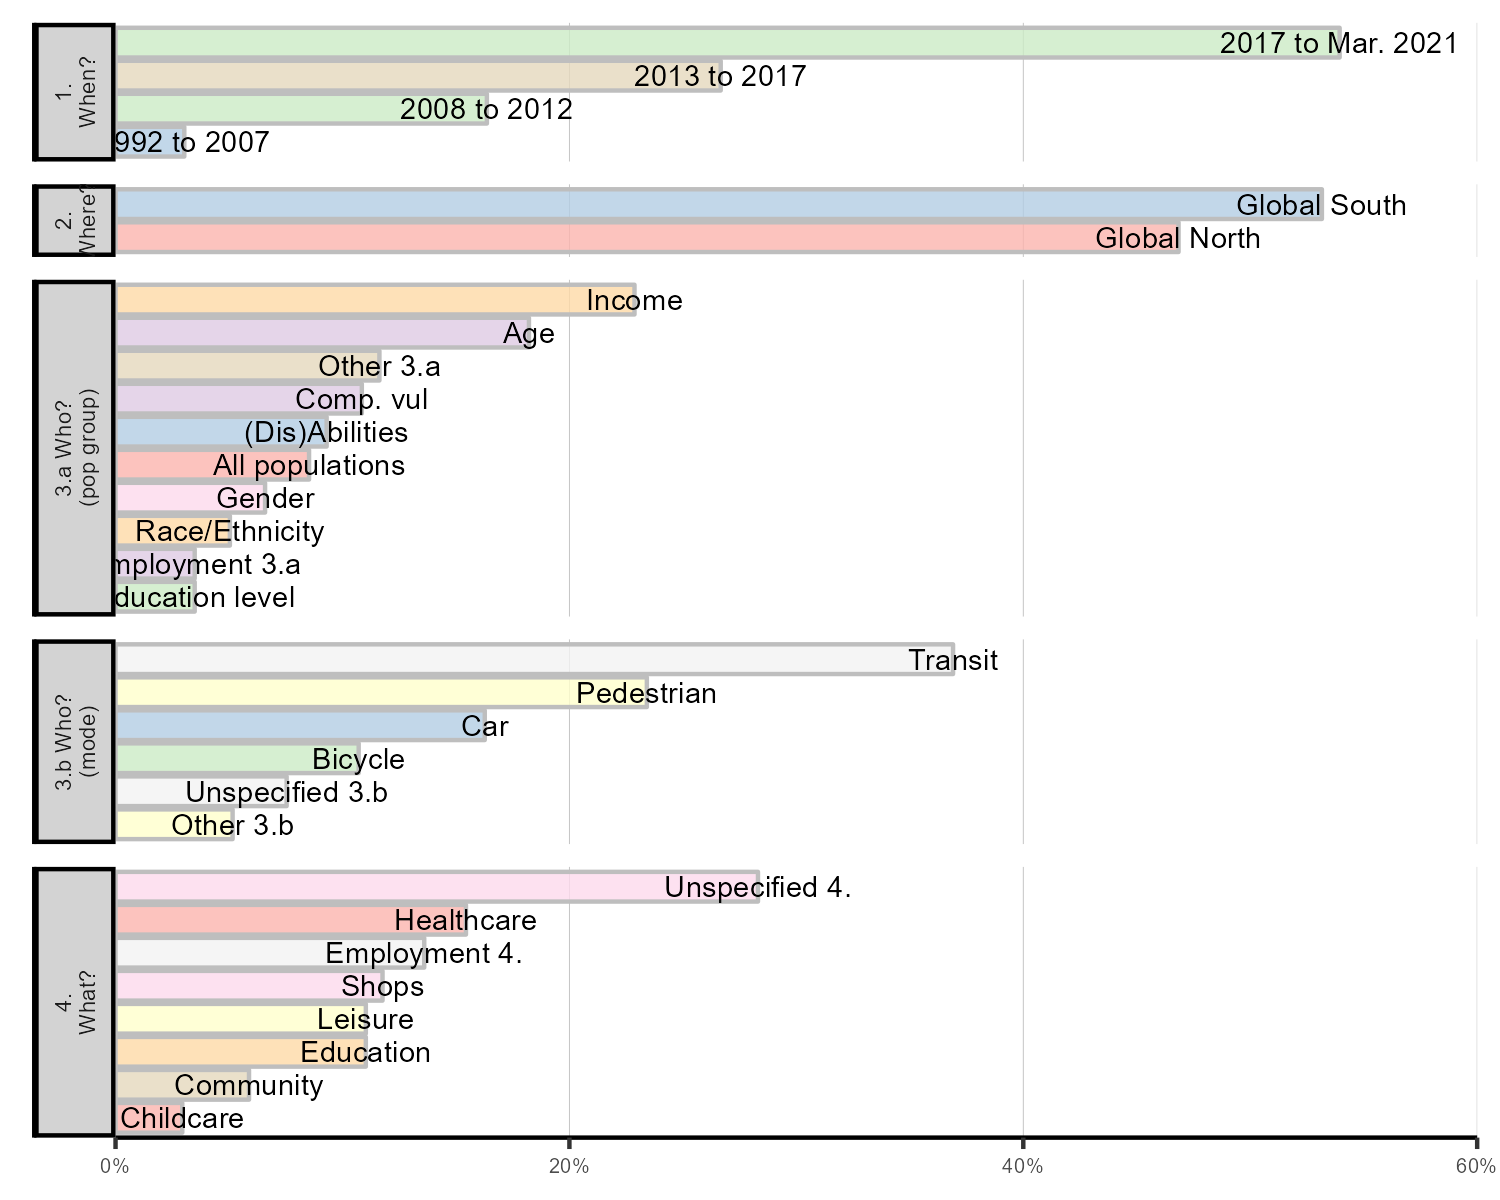
\includegraphics{figures/df_all_sub_ob_just_reordered_plot.tiff}

}

\caption{\label{fig-fig1}The proportion of papers in each `When',
`Where', `Who', and `What' by topics in each category. Topic categories
were generated by the authors based on the reviewed literature.}

\end{figure}%

\begin{figure}

\centering{

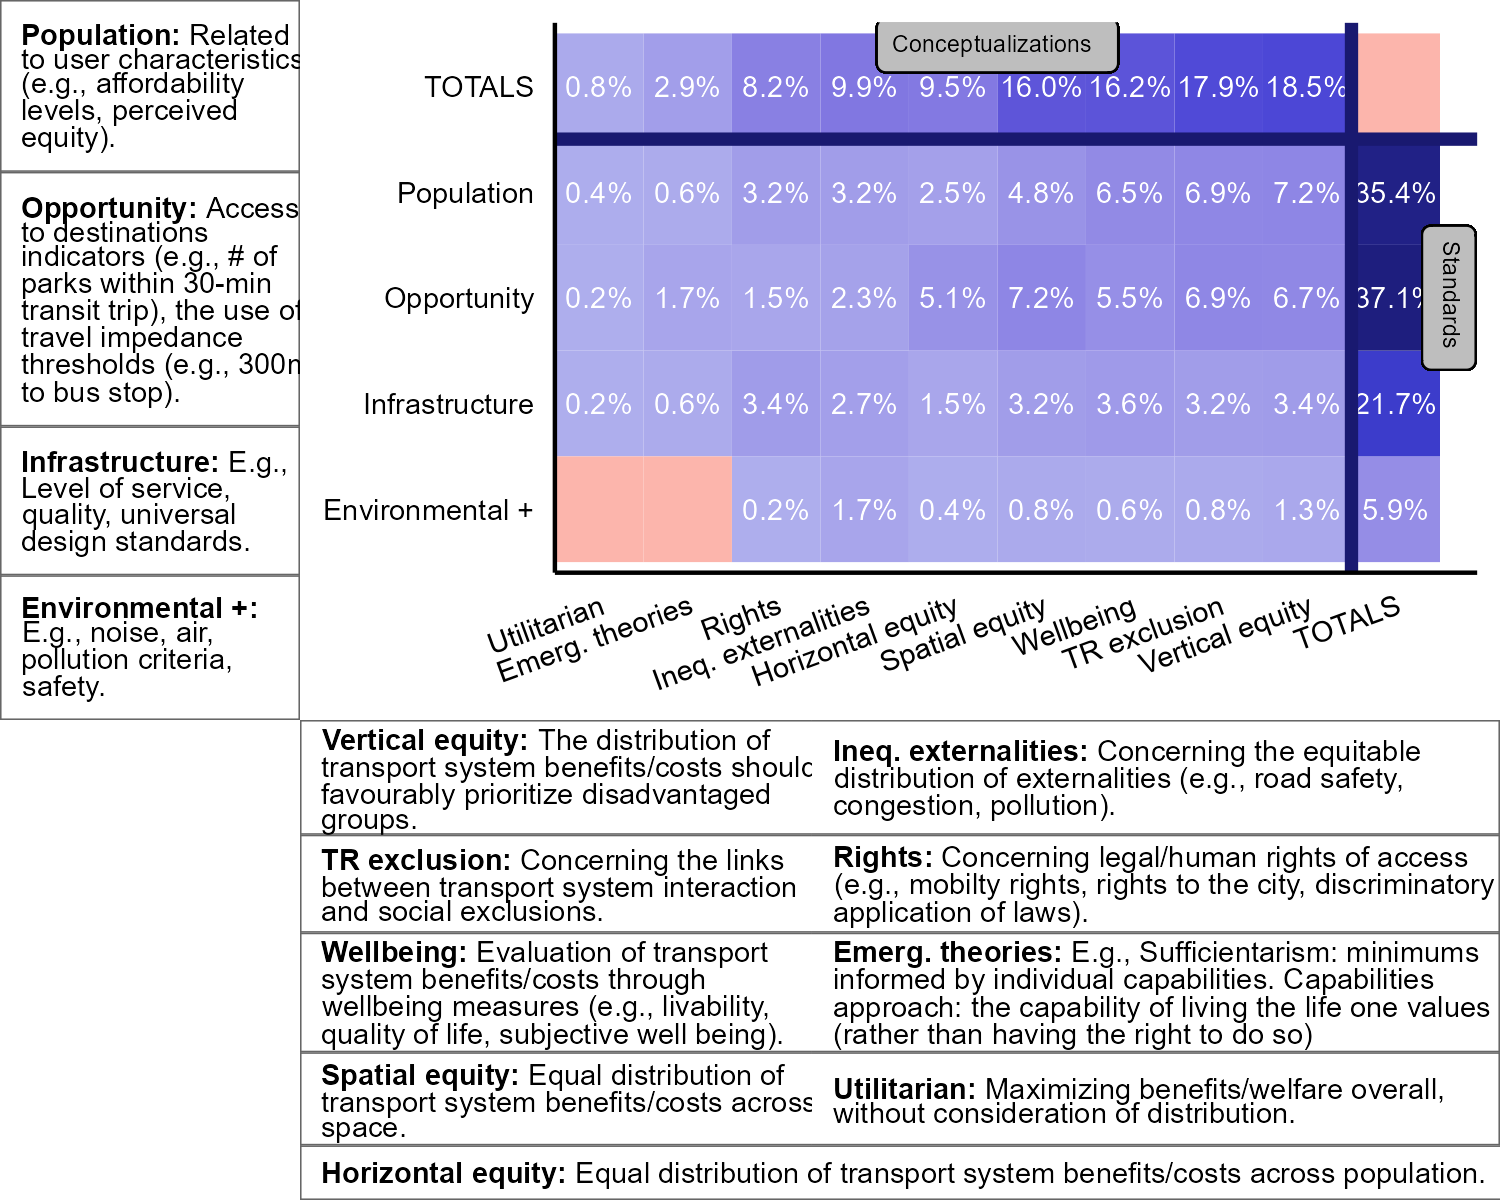
\includegraphics{figures/standards_conc_percentages_plot_and_table.tiff}

}

\caption{\label{fig-fig2}The proportion of papers by topics in the `How'
categories. `How' is split into two categories: topics related to
fairness conceptualisation (horizontal axis) and topics related to
standards (vertical axis). Topic categories were generated by the
authors based on the reviewed literature.}

\end{figure}%

\subsection{``When'' and ``Where'' is transportation fairness
considered}\label{when-and-where-is-transportation-fairness-considered}

Within our corpus, most papers (60\%) focus on studies in the Global
North, with many studies from North America (particularly U.S. and
Canada), Europe (France, Spain and Northern Europe), Oceania (Australia
and New Zealand), and Asia (Japan and Israel). Though their subject
matter is varied, their spatial context mainly pertains to North America
and Europe, and thus more often than not deals with more developed and
formal government transport planning apparatuses and technologies e.g.,
planning for equitable high-speed rail (Monzon et al., 2013), autonomous
vehicle technology (Eppenberger \& Richter, 2021), or on the public
consultation processes (Reddy et al., 2010).

Of note, work included in the reviewed literature does not often explore
the historical or temporal aspects of transportation fairness in depth.
Therefore, in this section we provide a thematic overview of the
temporal and spatial contexts associated with the studied case studies
and the publication location.

40\% of studies from the Global South are predominately from Asia,
notably China, but also India, Thailand, Iran, Philippines, and
Indonesia. The next most common focus within the literature from the
Global South is from South America. Many of these studies mention a
systemic absence of evidence relevant to the region (Vecchio et al.,
2020). Despite a growing recognition of the interconnections between
transport development, social exclusion, and poverty (Benevenuto \&
Caulfield, 2020), a number of studies underscore ongoing neglect of the
social dimension of transport during the planning stage (Benevenuto \&
Caulfield, 2020; Boisjoly et al., 2020). Many studies also point at
affordability as one of the main mobility barriers in the region
(Falavigna \& Hernandez, 2016; Rivas et al., 2018), while some highlight
multi-dimensional concerns such as public transport accessibility and
quality of walking environments that contribute to mobility inequalities
(Tiznado-Aitken et al., 2018). Studies pertaining to Africa are even
less numerous.

A shared characteristic among studies from Africa and South America is a
scarcity of official transport data (Fried et al., 2020). These studies
also incorporate the use of informal transportation options and tensions
in developing road network infrastructure (which tends to support car
dependency) over meeting the mobility/accessibility needs of citizens
more equitably and sustainably (Thondoo et al., 2020). To address these
challenges, researchers compile databases based on open and
geo-referenced data, calculate objective and/or subjective measures
(Berhe et al., 2014), and focus on advancing transport justice for low
to medium income countries by aligning their goals with external policy
guidelines such as the Sustainability Development Goals (SDG),
particularly those related to universal accessibility (Fried et al.,
2020).

Of all the studies reviewed, 85\% focus on urban and suburban settings
and are highly varied in their research aims. To give an example, Cox \&
Bartle (2020) qualitatively examine cycling as a mode of travel for
people with disabilities in a typical mid-size town in the U.K. Ampe et
al. (2020), on the other hand, work to identify the lateral clearance
that motorists should maintain when passing cyclists with children
seats. The remainder of the studies focus on rural regions (14\%), or
remote regions, such as those that rely on inter-island ferry trips in
the Philippines (Cao \& Stanley, 2017). Similarly, Parry et al. (2018)
studied remote communities in the Amazonian region, and suggest that
``increasing accessibility through road building would be maladaptive,
exposing marginalized people to further harm and exacerbating climatic
change by driving deforestation'' (pp.~125).

Overall, studies from the Global South often have some key differences
in focus compared to the Global North:

\begin{itemize}
\item
  affordability as a barrier at the user- or policy maker- level is more
  often the motivation in work from the Global South;
\item
  the expression of greater tensions in investing in new transportation
  infrastructure, such as roads in rural/under-developed areas, compared
  to prioritization of non-car modes. Studies centered in the Global
  North often focus on the later; and
\item
  more significant data availability limitations and reliance on
  `informally' collected data.
\end{itemize}

These differences center on the direct economic outcomes tied to
transport infrastructure. Often, work from the Global South does not
engage as intimately with emerging mobility technologies. As well, the
informal aspects of transport planning are more overbearing. Clearly,
countries in the Global South still struggle with the consequences of
past colonialism, which has left them more reliant on primary sector
exports (lower efficiency, lower national GDP) under growing global
financial markets, and with more fragile democracies. Due to lower data
availability, reliance on crowd-sourced or `informally' collected data,
and more extreme needs for `sufficient' transport, analysis of
transportation inequities is often cast along economic lines in the
Global South.

We gather that the literature on the Global North and South tend to
focus on different aspects of transport inequities, related to the level
of their transportation infrastructure. Formal planning processes in the
South operate under greater financial precariety, they rely on more
informal processes to address unmet needs. This turns out to be a
significant source of equity concerns, e.g, informal transit (Fried et
al., 2020), and populations living in informal settlements (Sharma \&
Patil, 2021). International standards are more highly relevant in
literature from the Global South, such as the WHO noise and air
pollution standard (Apparicio et al., 2021), while not as frequently
featured in the Global North literature. For example, in Carrier et al.
(2014), disadvantaged populations are disproportionately impacted by
higher \(NO_2\) pollution near roadways in Montreal, but these levels
are still consistently below the WHO standard. This difference in focus
presents interesting opportunities for the Global South, to adopt
potentially successful enhancements from Global North formal equity
planning processes (e.g., indicator creation for disadvantaged groups
(Cui et al., 2020)) and to avoid past and ongoing mistakes (e.g., from
entrenched car-centric development (Warren et al., 2015) to the
disproportionate contribution to carbon-intense mobility (Chancel \&
Piketty, 2015)). For the Global North, there is an opportunity to reckon
with its own contributions to uneven development globally and
environmental impacts as well as adopt relevant aspects from informal
planning processes.

\subsection{``Who'' are the subjects of transportation justice and their
mobility
tools}\label{who-are-the-subjects-of-transportation-justice-and-their-mobility-tools}

\subsubsection{Population groups}\label{population-groups}

Turning to the question of ``Who?'' in Figure~\ref{fig-fig1}, the focus
of the literature tends to be on ``Income'', especially the
lowest-income groups who simultaneously face lower mobility and
accessibility \emph{and} higher costs and exposure (Falavigna \&
Hernandez, 2016; Peungnumsai et al., 2020; Zhao et al., 2020). Evidence
suggests that low household income is a significant determinant of
transport-related inequities e.g., urban access to public transport
(Peungnumsai et al., 2020), access to urban employment opportunities
(Boisjoly et al., 2020), and unfavorable rates of environmental noise,
air pollution, and green space (Kruize et al., 2007). Yet, low-income is
not universally associated with lower transport-related benefits for
every object of justice. For instance, in Sheffield, U.K., Mears et al.
(2019) demonstrate that historically working-class (lower-income)
neighbourhoods have \emph{more} access to green space than other
neighbourhoods, but of lower quality, likely due to historic urban
planning approaches. Similarly, Bertrand et al. (2008) find that the
granularity of the analysis matters, and lower income groups do not
always have lower accessibility, something echoed in other spatial and
temporal contexts (Allen \& Farber, 2019; Foth et al., 2013)

``Age'' is the second most common ``Who?'' focus. In this regard,
Martinez-Jimenez \& Salinas-Perez (2019) and Arranz-Lopez et al. (2019)
investigate travel distances/times to various opportunities,
demonstrating how age is associated with differences in opportunity
access. School-aged children and older populations are a common focus.
For children, analysis of wellbeing (Laszkiewicz \& Sikorska, 2020),
safety and access to schools (Corazza et al., 2020; Sharma \& Patil,
2022), and promoting active travel (Mackie, 2009; Mehdizadeh et al.,
2017) are common-place. Papers that focus on older adults similarly
investigate transport-related wellbeing (Y. Chen et al., 2020), access
to age-specific destinations (Cheng et al., 2019), and options to reduce
unmet travel needs (Nordbakke \& Schwanen, 2015).

Many papers focus on intersecting characteristics. As an exception, we
classify some studies as focusing on ``(Dis)abilities'' or ``All
Populations''. Studies with a ``(Dis)abilities'' focus assess travel
capabilities, namely through physical accessibility and universal design
guidelines (Chiscano, 2021; Orellana et al., 2020; J. Park et al.,
2017). ``All Populations'' papers make no distinction in population.
This is done, for instance, by Kita et al. (2020), who investigates
disparities in accessibility to food stores and self-reported
capability/frequency of going outdoors. Often, the implicit or explicit
motivation of these papers is access (to necessities and desired
destinations) for all.

A large proportion of papers apply composite vulnerability indices that
combine several individual traits like low income, unemployment, and/or
immigrant status. These indices are generated from government sources or
author-informed census data creation methods. As an example, the
Neighbourhood Equity Index is a measure of vulnerability created by the
City of Toronto and used in Awuor \& Melles (2019) to examine
disparities in premature death. Other works use national census
indicators such as the social and housing deprivation index (Pucci et
al., 2019) or explore transport disadvantage, equity in policy
implementation, or transport-related mortality burden by means of census
measures (e.g., household poverty) and transport-related accessibility
indicators (Aldred et al., 2021; Iungman et al., 2021; Scheurer et al.,
2017; Sun \& Thakuriah, 2021). Similarly, Environmental Justice (EJ)
indicators have been used in the U.S. literature to identify
neighbourhoods that have a higher than average proportion of low-income
and non-white populations and evaluate the equity impacts of
transportation projects (K. Park et al., 2021; Reddy et al., 2010;
Rowangould et al., 2016).

Multi-dimensional considerations are so prevalent in the reviewed
literature that ``Gender'', ``Race/ethnicity'', ``Education'', or
``Employment'' are infrequently studied in isolation. Only a few papers
focus exclusively on gendered differences in active transportation
(Adlakha \& Parra, 2020; Xie \& Spinney, 2018), race/ethnicity's
relationship to green space proximity (Silva et al., 2018), and
culturally-appropriate opportunities (Wang \& Roisman, 2011). Papers
that focus \emph{solely} on ``Employment'' status or ``Education'' level
are completely absent in the corpus. Furthermore, ``Other'' population
groups are also frequently considered: this is a catch-all category that
includes populations less commonly targeted by research e.g., veterans
and access to specific-healthcare needs (Mooney et al., 2000), pregnant
people and access to maternity services (Vadrevu \& Kanjilal, 2016), and
youth who live in foster care (Batsche \& Reader, 2012). Overall, the
diversity of population groups considered in the corpus demonstrates the
variety of transportation-equity concerns addressed.

\subsubsection{Modes (mobility tools)}\label{modes-mobility-tools}

Travel mode, though modifiable, is intertwined with individual identity,
presenting challenges for the analysis of disparities. In this
subsection, we choose to view the mode of travel primarily as those who
use the mode, hence as subjects of justice (i.e., the ``Who?'').
However, at times, travel mode will also be considered as an object of
justice (i.e., a ``What?'', such as disparities in rural transit
service).

To begin, transit characterises the majority of the reviewed literature
(Figure~\ref{fig-fig1}), reflecting some intuitive sense. Despite
transit being perceived unfavourably by some (e.g., Mella Lira \& Paez
(2021)), it is often viewed as the only or primary mobility option mode
for many (Jacques et al., 2012). Overall, we can infer that transit is
largely considered a public good and, therefore, a natural object of
justice. As such, public transportation is especially amendable to being
modified to meet the demands of justice by ensuring adequate funding to
provide barrier-free transport for most, despite challenges such as low
densities, fiscal constraints, and political will (Markard et al.,
2023). As such, papers that focus on transit assess a variety of related
topics, including food deserts (McKey et al., 2020) and barrier-free
transportation for people who face disabilities (Feeley, 2019;
Jiménez-Espada \& González-Escobar, 2021; Lim et al., 2021; Liu et al.,
2019).

Transit also plays a central role in multimodal comparisons in transport
disparities, especially comparing ``Walk'', ``Car'', or some other
category in Figure~\ref{fig-fig1}. For instance, Brussel et al. (2019)
compares transit, pedestrian and road network accessibility measurements
in the context of SDG 11.2. Renne \& Mayorga (2018) reviews natural
disaster evacuation plans, focusing on carless households and
emphasizing transit and pedestrian networks. A few papers also frame
transit as a direct competitor of car travel or use it as a benchmark
(Golub \& Martens, 2014; Martens et al., 2012). For instance, Warren et
al. (2015) proposes car ownership standards while acknowledging the
tension between mobility needs in transit under-served areas and
emission reduction goals. However, this framing is not universal, and
transit is sometimes seen as a mode to fulfill individual capabilities.
As an example, Smith et al. (2012) explores perspectives about transport
needs and costs to achieve perceived sufficient living standards for
those living in rural areas. Notably, papers vary in the importance they
place on climate urgency, with some focusing more on satisfying
\emph{all} sufficient individual needs while planning for less
car-dependent cities in the future.

After transit, pedestrian travel (``Walk'') is the second most studied
object of justice. Pedestrians represent a unique convergence of
``what'' and ``who,'' utilizing their own bodies for mobility. Papers
focusing primarily on walking often use walkability scores to assess
neighbourhood quality (Evans, 2015), mobility by different demographics
(H. Kim et al., 2016; Towne et al., 2016), or urban peripheral regions
(Blecic et al., 2021). Some use walkability to gauge public health and
urban vitality (McCormack et al., 2012; Sung \& Lee, 2015). Papers with
a pedestrian focus also often see walking as a bridge to connect
multiple modes: they discuss `walkability' as part of active
transportation, which focuses on both walking, bicycle and/or transit.
Concepts discussed include how active transport contributes to
children's physical activity levels (Mammen et al., 2014), walkability
as an alternative to car predominance (Bertrand et al., 2008) or tension
that exists between modes, creating unsafe conditions for walking
(Ferenchak \& Marshall, 2019; Siu, 2019).

The third most studied mode in the reviewed literature is ``Car''.
Unlike transit and walking, these studies rarely feature car as the mode
of primary focus. Car is often assessed against transit and active modes
(e.g., low traffic neighbourhoods Aldred et al., 2021) or in areas with
inadequate transit service (Aljoufie, 2016; Kimmel et al., 2018). Under
our appraisal, transit and walk modes are of most interest because they
represent a reckoning with automobility's legacy and ongoing demands for
space, public subsidies and government supports that underestimate their
true cost (Gössling et al., 2019; Timperley, 2021). Upon the rise of the
automobile, pedestrian spaces were distinguished, non-car modes came to
be seen as a hindrance to full automobility, and transit seen as a
social service. We ascertain that for these reasons, ``Car'' is often
compared against non-car modes and never put forward as the only mode
that should be expanded. Furthermore, some papers reflect on ``Other''
forms of mobility (Figure~\ref{fig-fig1}), including
wheelchair-accessible taxi and/or paratransit services (Marquez et al.,
2019; Wilkinson-Meyers et al., 2015), travel on waterways (Cao \&
Stanley, 2017; Parry et al., 2018; Vadrevu \& Kanjilal, 2016),
motorcycle or other micro-mobility (Berry et al., 2016; Schmitz et al.,
2019; Tiwari \& Phillip, 2021), or emergency vehicles (Patel et al.,
2007; Pedigo \& Odoi, 2010).

Papers that pay no particular attention to any mode are ``Unspecified'':
as examples, a focus on road infrastructure or road network distances
(Mishra et al., 2014; Wismadi et al., 2014), travel needs generally
(Benevenuto \& Caulfield, 2020; Titheridge et al., 2008), realized
travel (Abasolo et al., 2001), or externalities of realized travel
(Iungman et al., 2021).

\subsection{``What'' could be the objects of transportation
justice}\label{what-could-be-the-objects-of-transportation-justice}

The objects of fairness assessment, the ``What'', are often motivated by
concepts encompassed by either mobility or accessibility. A fundamental
benefit of transportation systems is mobility (enabling or impeding
movement). This benefit is sometimes valued by itself but is often seen
by the literature as instrumental to achieve an ulterior goal (e.g.,
activity participation and associated benefits). For example, although
vehicle kilometers traveled (VKT) is sometimes seen as a useful policy
instrument (Zhao \& Li, 2021), travelling more is not necessarily a sign
of advantage when accessibility is low, and short trips may actually be
a sign of advantage (K. Park et al., 2021). For this reason, although
the right to the road (and transportation systems more generally) is
important, the literature leans heavily on the ulterior object, namely
accessibility to (the ease of reaching) destinations. In tandem, themes
of existing transportation system burdens associated with mobility and
accessibility can be interpreted: for instance, these could be
environmental (e.g., potential for GHG emissions reductions relative to
the status quo (Bocarejo \& Urrego, 2022)), or human-health and
traffic-related externalities (e.g., decreased wellbeing due to
transport poverty (Churchill \& Smyth, 2019) or reduction in potential
road-related fatalities (Bocarejo \& Urrego, 2022))

\subsubsection{Mobility}\label{mobility}

Most papers in the reviewed literature take a broad approach, with 47\%
focusing on ``Unspecified'' destinations (Figure~\ref{fig-fig1}),
examining various equity dimensions across different transportation
modes. Many of these papers are `mobility' focused and examine the
impact of the trip itself on the individuals, groups or the environment.
These benefits and burdens include safety (Zhe et al., 2008),
infrastructure quality and service levels (Fürst \& Vogelauer, 2013;
Lattman et al., 2016; Prasertsubpakij \& Nitivattananon, 2012) or air
and pollution levels (Apparicio et al., 2021). Others analyze trips
taken by specific groups like women or people with disabilities (Russell
et al., 2021; Wilkinson-Meyers et al., 2015), often with a consideration
of what constitutes `sufficient' quality of life (Churchill \& Smyth,
2019). In sum, these papers reveal the multifaceted nature of
transportation systems: they serve utilitarian purposes related to
travel while also shaping user experiences, expressing some aspects that
can be summarized as societal and/or planetary benefits and burdens.

\subsubsection{Access to opportunities}\label{access-to-opportunities}

Generally, papers that focus on a particular destination can be
construed to interpret ``accessibility'' as the ``What?'' as the object
of fairness, with access \emph{to} opportunities being the benefit. When
analyzing access to particular destinations, ``Healthcare'' services
(18\%) and ``Employment'' (25\%) are the most common in the reviewed
literature (Figure~\ref{fig-fig1}). Papers on healthcare often highlight
disparities in services, like Wang \& Roisman (2011), who assess access
to Mandarin speaking family physicians for Mainland Chinese immigrants
in Toronto. Similarly, papers focusing on employment are often aimed at
identifying transportation-poor neighbourhoods (Allen \& Farber, 2019;
Churchill \& Smyth, 2019). Employment is frequently used as a proxy for
overall accessibility since it is the most common trip purpose and
employment is usually co-located with destinations like shops,
recreation, and other services. These studies typically use travel
surveys, census data, and point-of-interest databases, and benefit from
well-developed institutional data. This especially holds in the Global
North where these data are more readily available.

Other destinations have received less attention despite serving
essential needs. ``Shopping'' destinations (19\%) often aim to identify
food deserts (Choi \& Suzuki, 2013; Jiao et al., 2012; D. Kim \& Park,
2020; McKey et al., 2020). ``Education''-related papers (18\%) explore
children's active transportation to school (Larkins et al., 2011) or
universal design (Larkins et al., 2011). Places of ``Leisure'' (18\%)
prompt questions about their spatial distribution (M. Xu et al., 2017)
and accessibility (Mavoa et al., 2015). Fewer papers cover ``Community''
destinations (e.g., public service centres, places of community support
or worship) (10\%) or ``Childcare'' (5\%), but they are integral to
holistically study activity participation (Alberts et al., 2016; Smith
et al., 2012). The lack of information about community destinations in
the reviewed literature, especially for children, is noticeable
(Desjardins et al., 2022). In sum, these works that focus on
`accessibility' can be seen to frame access and its related
externalities as benefits, while the lack of access (or associated
externalities) as burdens.

\subsection{Standards: ``How'' fairness is
measured}\label{standards-how-fairness-is-measured}

\subsubsection{Conceptualisations of
fairness}\label{conceptualisations-of-fairness}

The conceptual foundations of fairness are often not made explicit
within the reviewed literature, they have to be inferred. Though not
exhaustive, the following categories emerged from our review and in
broad terms are (Figure~\ref{fig-fig2} details definitions):

\begin{itemize}
\item
  Vertical equity (27\%)
\item
  Transport-related social exclusion (27\%)
\item
  Well-being (27\%)
\item
  Spatial equity (26\%)
\item
  Horizontal equity (17\%)
\item
  Inequitable externalities (17\%)
\item
  Rights (14\%)
\item
  Emerging theories (5\%)
\item
  Utilitarian (1\%)
\end{itemize}

A slice of the reviewed literature is supported by broader ``Rights''
conceptualisations of fairness: these papers often focus on equity for
people with disabilities or non-car users and associated challenges
accessing transport infrastructure (Bharathy \& D'Souza, 2018; Daamen et
al., 2008; Jiménez-Espada \& González-Escobar, 2021). While many papers
are underpinned with the right to the city (the \emph{right} to
participate in the production of urban space (Adli \& Donovan, 2018;
Lefebvre, 1967)), others emphasize legal \emph{Rights} like regulations
aligned with The Americans with Disabilities Act (ADA) (Bharathy \&
D'Souza, 2018) or the goal of \emph{access for all} in land-use
transportation master plans (Lim et al., 2021).

In another subset of the reviewed literature, distributions are examined
through concepts of ``Horizontal'' and ``Spatial equity'', often using
quantitative methods to assess distributional disparities without
explicit justice rationales. Examples include setting travel impedance
thresholds (Shen et al., 2020) and mapping accessibility indices
spatially across populations (Monzon et al., 2013) or population-groups
(Sharma \& Patil, 2021). These papers may also address burdens such as
traffic-related air and noise pollution or urban temperatures. In these
papers, equity is theoretically achieved if similar levels are attained
for all populations (horizontal equity) or spatial areas (spatial
equity). This egalitarian perspective rarely delves into minimum or
maximum levels associated with harm or need satisfaction.

Papers that center ``Well-being'' assess what constitutes a satisfactory
life in relation to transportation; mixed-methods are often used and, in
contrast to the last set, the objects of injustice are often identified.
Some papers use physical activity guidelines and surveys to understand
the effect of active transportation infrastructure (Adlakha \& Parra,
2020; Auchincloss et al., 2020; McCormack et al., 2012). Mixed or
qualitative methods combined with health-related outcome standards lead
to more concrete statements of fairness e.g., travel times for emergency
treatment (Schmitz et al., 2019) or premature mortality (Awuor \&
Melles, 2019).

Another research branch, often quantitative with some qualitative or
mixed-methods studies, focuses on ``Transport-related social
exclusion'', ``Vertical equity'', and/or
``Sufficientarian/capabilities''. Here, the objects of justice are often
clearly identified and link standards to tangible welfare-informed
outcomes. They focus on groups from perspectives of disadvantage such
as: social exclusion and transport poverty (Allen \& Farber, 2019;
Churchill \& Smyth, 2019; Delbosc \& Currie, 2011a), food deserts (McKey
et al., 2020), and energy poverty (Berry et al., 2016; Berry, 2019;
Robinson \& Mattioli, 2020).

\subsubsection{Standards and methods of measuring
fairness}\label{standards-and-methods-of-measuring-fairness}

We identify several categories of standards that overlap with at least
one of the conceptualisations of fairness discussed above (see
Figure~\ref{fig-fig2} for definitions):

\begin{itemize}
\item
  Opportunity standards (66\%)
\item
  Population standards (64\%)
\item
  Infrastructure standards (41\%)
\item
  Environment+ standards (7\%)
\end{itemize}

Papers with ``Opportunity'' standards often employ quantitative methods
to analyze disparities and assess distributional fairness. Many deal
with travel impedance thresholds based on speed, distance, or cost (Z.
Chen \& Haynes, 2017; Shen et al., 2020; Yenisetty \& Bahadure, 2020).
Inequality measures like the Gini coefficient and poverty measures are
used to empirically define travel impedance thresholds (Tiznado-Aitken
et al., 2018; van der Veen et al., 2020). Further, methods tangential to
travel impedance, like limiting transport expenditure to 10\% of monthly
income (Rivas et al., 2018), addressing spatial mismatch (Mulley et al.,
2015), or pinpointing areas of relative regional inequities are also
used. Notably, many papers with ``Opportunity'' standards consider
multiple dimensions, employing similar methods but tailored to different
focal points. For instance, Peungnumsai et al. (2020) suggest service
benchmarks of equal supply and demand of transit, revealing horizontal
inequities as well. Others conceive the externalities of transportation
system as trade-offs and aim to maximize transport-related benefits
(i.e., time savings, emissions reductions, congestion reductions, user
fares) through optimization/location-allocation methodologies
(Fakhrmoosavi et al., 2021; Wismadi et al., 2014; Zheng \& Geroliminis,
2020).

``Population'' standards are often founded on ``Well-being''
conceptualisations from a variety of socio-demographic and spatial
angles. Methods include: establishing thresholds based on questionnaires
and comparisons to recommended physical activity levels (Auchincloss et
al., 2020; H. Kim et al., 2016; McCormack et al., 2012; Timperio et al.,
2015), region-relative comparisons in health outcomes in a spatial unit
such as premature mortality rates (Awuor \& Melles, 2019), spatial
access benchmarks based on population-related characteristics like
supermarket access (Murphy et al., 2017) and hospital access (R. Pereira
et al., 2021), summative per capita benchmarks such as decent living
energy consumption levels (Rao \& Baer, 2012), and community-informed
spatial boundaries like EJ defined communities (Rowangould et al.,
2016). While most of these papers use quantitative or mixed-methods
approaches, some employ exclusively qualitative methods (Berhe et al.,
2014).

Papers that feature both ``Population'' and ``Opportunity'' standards
are often founded on ``Vertical equity'', ``Well-being'', and/or
``Transport-related social exclusion'' conceptualisations. They feature
mixed-methods, with questionnaires and qualitative approaches for
``population'' standards and quantitative methods like accessibility
indices for ``opportunity'' standards. Census data and household
estimates within specific travel distances or times to key destinations
identify social exclusionary situations (W.-H. Chen, 2010; Daniels \&
Mulley, 2011; Sharma \& Patil, 2021; Sun \& Thakuriah, 2021), linkages
between transport disadvantages (Delbosc \& Currie, 2011a), areas
experiencing transport poverty (Allen \& Farber, 2019; Churchill \&
Smyth, 2019), food deserts (McKey et al., 2020), or transport-related
energy poverty (Berry et al., 2016; Berry, 2019; Robinson \& Mattioli,
2020). They employ various methods, such as clustering techniques (Mohri
et al., 2021). Some exclusively use qualitative methods to analyze
survey data on travel willingness/barriers or conduct interviews on
unmet activity needs (W.-H. Chen, 2010; Mehdizadeh et al., 2017;
Nordbakke \& Schwanen, 2015).

``Infrastructure'' standards offer another perspective on fairness,
commonly grounded in ``Rights'' conceptualisations, which are twice as
frequent in this segment of the corpus compared to other
conceptualisations. These papers most frequently address the rights of
non-car users and populations with disabilities. Though various methods
are applied, infrastructure and environmental audits as well as
qualitative approaches are most prominent. Infrastructure audits compare
existing infrastructure against universal design best practices
(Jiménez-Espada \& González-Escobar, 2021; Larkins et al., 2011; Odeck
et al., 2010; Perez-delHoyo et al., 2021) or investigate elements
correlating with mode use by specific population groups (Moniruzzaman \&
Paez, 2016). Qualitative methods include interviews/surveys on perceived
access (Desjardins et al., 2021; Fürst \& Vogelauer, 2013; Lim et al.,
2021; Marquez et al., 2019; Mateo-Babiano et al., 2017; J. Park et al.,
2017; Stjernborg, 2019; Velho et al., 2016) and assessment of standards
under best-practice criteria (Bharathy \& D'Souza, 2018; Daamen et al.,
2008; Velho et al., 2016).

Additionally, ``Infrastructure'' standards papers sometimes encompass
multiple dimensions, moving beyond rights (to the infrastructure) to
provide ``Opportunity'' and/or ``Population'' standards. These papers
often employ ``Vertical'', ``Horizontal'', and ``Spatial equity''
lenses. These papers often refer to guidelines and propose composite
indices. For example, (Rachele et al., 2017) integrate various transport
network properties to define an indicator supporting walkability and
public transport access. Others evaluate infrastructure quality (M. Xu
et al., 2017), accident severity (Appleyard et al., 2017; Benevenuto \&
Caulfield, 2020), and user-groups, especially disadvantaged ones with
respect to vertical equity of multi-criteria indicators (Prasertsubpakij
\& Nitivattananon, 2012). Some focus explicitly on affordability and
barriers, proposing infrastructure enhancements for better inclusivity,
especially for the most disadvantaged (Basu \& Alves, 2019; Song et al.,
2019; Welch, 2013), grounded in transport-related social exclusion (Kent
\& Karner, 2019) or capabilities approaches (Smith et al., 2012).

``Environmental+'' standards are featured less prominently in the
reviewed literature, possibly because the environmental burdens of
transportation are addressed more broadly in other literature (e.g.,
environmental justice). However, the papers included in our corpus
present some interesting insights. They often use traffic-related air
and noise pollution, green space, urban design, urban air temperature,
health outcomes, and physical activity guidelines to assess
transport-related ``inequitable externalities''. Methods employed are
primarily quantitative or mixed-methods, identifying inequalities
through Gini coefficients (Feng \& Timmermans, 2014) or composite
indices (Agost-Felip et al., 2021; Corazza et al., 2020; Miranda \& da
Silva, 2012), occasionally incorporating spatial analysis (Carrier et
al., 2014; Jephcote \& Chen, 2013). Many use established thresholds or
health guidelines e.g., WHO guidelines for Active Aging and targets
included in the United Nations' SDG (Agost-Felip et al., 2021) and OECD
or WHO standards for traffic noise level, \(NO_2\) levels, available
green space and \(PM_{2.5}\) levels (Apparicio et al., 2021; Iungman et
al., 2021; Khomenko et al., 2020; Kruize et al., 2007; Mueller et al.,
2018). These metrics are sometimes criticized for their general
applicability. Nonetheless, their use provides interpretable values for
tracking progress, offering comparability across communities, unlike
accessibility measures, which vary in methods and assumptions.

Appendix Section~\ref{sec-sect63} presents detailed examples of various
standards, outlined within the 5WH framework, as derived from the
examined corpus.

\section{Moving forward: discussion and calls for
action}\label{moving-forward-discussion-and-calls-for-action}

As previously noted, this work makes two contributions to the
literature. First, it outlines a conceptual and flexible ``Why'',
Where'', ``When'', ``Who'', ``What'' and ``How'' (5WH) framework with
supporting definitions for approaching questions about transportation
justice. Second, it applies the framework in synthesizing and appraising
of 165 academic articles drawn from the transportation justice
literature; these studies use equity analysis as instruments to gauge
proximity to their context's just situation. Based on the preceding
sections of what is in the literature, and what is lacking from our
perspective, we conclude with the following five calls to action. Based
on the preceding sections of what is in the literature, and what is
lacking from our perspective, we conclude with the following five calls
to action.

\subsection{Call 1: Underpin tailored standards based on rigorous
concepts of
justice}\label{call-1-underpin-tailored-standards-based-on-rigorous-concepts-of-justice}

The conceptual grounding for standards is often left implicit within the
literature. For example, Mueller et al. (2018) suggests the relative
risk of mortality from transport-related air pollution should not be
higher in deprived groups than the general population. While the
conceptual justice foundations are not explicitly declared, we infer an
egalitarian focus. But, what level of relative risk is acceptable for
the general population? What purpose does mortality risk serve and who
benefits from it? To move equity analysis outputs towards just transport
futures, explicit inclusion of justice rationales (the ``Why?'') should
become more common place. We must be clear with our terms--what is
equity and for whom?

Standards are statements of fairness, yet some standards are seemingly
arbitrary in the reviewed literature--in other words, set arbitrary
justice goals. For example, Cao \& Stanley (2017) proposes 20 ferries
per day to avoid social exclusion for inter-island transport planning,
though acknowledging the standard should be politically determined. It
is unclear if selecting a different benchmark such as 10 or 30 ferries
would make a difference in any specific object of justice (e.g.,
accessibility to particular destinations) or if that number is tied to
funding or resource constraints. Another example is the conceptual
underpinnings of the 15-minute city, where 15 minutes is the standard
for travel times. Is this sufficientarism? Or egalitarianism? The
standard can be interpreted in a multitude of ways. We argue that
conceptualization of justice must guide the selection of the standard.
As Martens \& Golub (2021) demonstrate, being explicit about ``Why'' is
important. Recent work by Karner et al. (2024) provides several concrete
examples for developing standards that follow directly from different
justice conceptualizations.

Additionally, there is a need to go beyond the focus on low-income
transit riders, as clear ``Who?''-specific standards are lacking.
Positioning intersectional considerations within the creation of
community-based equity definitions and tailored standards are critical,
as the act of delineating equity-deserving communities impacts results
(e.g., Rowangould et al. (2015)). Standards should be sensitive to
evolving community-based definitions of inequities. Are issues of
economic inequity at the root of transport inequities for a particular
community? Are inequities in access provided by certain modes emphasized
because access offered by other modes are \emph{relatively} better?
Access to what types of opportunities are driving transport inequities?
How do populations, travel modes, and opportunities sought intersect to
define the ``who'' of inequities? A community-informed understanding of
inequities and tracking how they change are needed.

For decision-makers, setting standards, measuring inequities, and
developing flexible guidelines for standards that are also compatible
with community-informed calls for justice, are the next steps for
transportation equity planning. If we assume that one function of the
academic literature is to recommend standards, researchers must connect
compatible conceptualisations and standards to justice frameworks.
Currently, these fundamental connections are mostly missing.

\subsection{Call 2: Develop creative methods for systems-thinking
approaches to
fairness}\label{call-2-develop-creative-methods-for-systems-thinking-approaches-to-fairness}

On the methodological side, transportation justice research would
benefit from a wider use of mixed-methods. Concepts and standards are
often discussed from purely qualitative or quantitative approaches. This
is a missed opportunity to combine the strengths of both approaches,
whether by diving deeper into some particular experiences or perceptions
through qualitative methods or tailoring more meaningful quantitative
analysis after qualitative explorations. As mixed-method examples, Xie
\& Spinney (2018) find through interviews and go-alongs with women
cyclists that the standard Cycling Level of Service tools used by
engineers to plan cycling infrastructure misses a critical gendered
perspective. Further, Somenahalli \& Taylor (2007) survey older adults
to understand their mobility issues, revealing factors that are unseen
in standard daily travel surveys.

While disparity analysis is frequently used, the resulting standards do
not often align with practical applications. For example, metrics of
accessibility (usually measured with travel impedance cut-offs of
between 15 to 60 minutes depending on the destination, population group
and mode) are used to show descriptive differences among areas and
groups but with scarce implications as to the experience of travelers.
How low must an accessibility index be before it is too low? Relatedly,
once sufficient accessibility levels are reached, excessively high
accessibility values can result in high inequalities. Are inequalities
of a certain level an issue? A lack of discussion poses a challenge to
translating results from these analyses into policy and practice.
Creative methods and discussions of quantitative accessibility metrics
should be paired with results; they should yield interpretable results.
The explicit discussion of minimum \emph{and} maximum values in the
distribution of the object of justice (the ``What?''), as applicable, is
critical.

Other times, when analysis engages with metrics that may be tied to
particular concepts of equity (like the Gini coefficient or Theil
index), they fall short in assessing whether the results are good or bad
(Mijares et al., 2013). For example, a Gini coefficient of 0 would mean
that all people have the same access to public transport stops. But is
this level of access good enough or lacking? And what does it mean if
the result is 0.2, 0.3, or 0.4? Is this good or bad news? How should a
decision-maker interpret this? Are new policies needed to reduce that
number to a certain threshold, orienting future interventions? These
questions usually remain unanswered in the literature despite their
importance. These measurements can also bring some challenges and
pitfalls as summarised by Karner et al. (2024) but are necessary for
more effective equity analyses.

\subsection{Call 3: Making data available is a matter of
justice}\label{call-3-making-data-available-is-a-matter-of-justice}

In our review of the literature, we were left wondering specifically--
what are the motivations for the inclusion of some destinations and the
choice to not include others? For instance, leisure (e.g., green space,
parks, recreation) and certain care destinations (e.g., community
organizations, government services, banking locations, daycares) are
infrequently studied or missing altogether. We suspect that since the
methods used in the reviewed literature are predominately quantitative,
the reliance on commonly used point of interest databases is also high.
These databases typically include education, health, and occasionally
include aggregated categories for leisure and community destinations,
but are less generous for points of interest that are more often
associated with understudied mobility patterns.

However, through the reviewed literature, we know that transport systems
are more than just facilitators to work or as a source of economic
development (though in underdeveloped regions, transport systems as a
force of economic development is pronounced, e.g., high-speed rail (Z.
Chen \& Haynes, 2017; H. Kim \& Sultana, 2015; Monzon et al., 2013)). As
such, data availability matters. In the context of the Global South and
rural geographies fewer official data sources and public research
resources exist relative to urban communities and areas in the Global
North. The operationalization of emerging conceptual theories in equity
analysis, such as sufficientariansm (van der Veen et al., 2020), might
be impacted if relevant data is not available.

The calls for and relevant issues of data availability are not new, but
they have at least three pieces. What and who is the subject of justice?
When/Where/How is it measured? And, who gets to consult and use the
data? Deciding who is the subject of justice frames the data collection
activity; if it is the mobility of those who do domestic work, the
classification of who does this work and how it changes over time/space
is fundamental. How we classify mobility and access has implications for
our understanding of just who is a subject of justice, as illustrated by
the history of racial classifications in the U.S. (Lee, 1993). The
methods we use, the spatio-temporal boundaries for data collection, and
who has (and does not have) access to the collected data, can all impact
how we think about justice. In the case of transportation, the issue of
data collection/availability as a matter of justice is gaining traction
as digitization of data casts a starker light on these questions
(Behrendt \& Sheller, 2023; Sourbati \& Behrendt, 2021).

\subsection{Call 4: Develop more direct and explicit links between
standards and lived
experiences}\label{call-4-develop-more-direct-and-explicit-links-between-standards-and-lived-experiences}

Robust assessments of the implications of standards on lived experiences
are still lacking in the literature, but are essential for equity
analysis that translates into just practice. While the estimation of the
benefits of increased mobility or accessibility, or reducing burdens is
commonplace in the literature, there is a need to associate them with
outcomes, including life and neighbourhood satisfaction, subjective
well-being, mental and physical health, and social capital. The
literature must move beyond describing inequities and their contributing
factors. Instead, it should incorporate causal methods that establish
clear cause-and-effect relationships, enabling policymakers to quantify
the impact of various policies and infrastructure decisions on advancing
justice.

Composite measures such as the transport-land-use index proposed by
Appleyard et al. (2017) is an example of systems-thinking approach that
links findings to quality-of-life proxies; they ground their measure in
the principle of \emph{livability} along corridors of varying levels of
estimated transport-land-use integration. However, the methods could go
further: they could be tied to absolute goals of integration or
livability. Relatably, Higgs et al. (2019) develops an urban livability
index and demonstrates the relationship between the population's use of
a certain mode in a neighbourhood and a one unit increase in the index.
However, are there absolute minimums or maximums for the index or the
mode-choice goals that should not be crossed?

More explicit discussion of the boundaries in the distribution of the
object of justice (the ``What?'') alongside these creative methods are
needed. These links may be used to track progress towards justice across
time and space, a critical point for practitioners.

\subsection{Call 5: Rigorously evaluate interventions and
policies}\label{call-5-rigorously-evaluate-interventions-and-policies}

There is a need to evaluate equity interventions and policies: track
their before, during, and after. In this review, a small proportion of
studies assess specific transport-related policy interventions through
an equity lens. Examples include mode-shift from driving to active
school travel (Mammen et al., 2014), transit fare restructures (Hickey
et al., 2010) and spatial analysis of Low Traffic neighbourhoods (Aldred
et al., 2021). The assessment of interventions and tracking associated
outcomes can be thought of as a key step towards transport justice.
Similarly, for how long the burdens and benefits can still be associated
to a specific transportation intervention remains a critical avenue to
explore.

Outcomes of interventions can be compared within and between
communities, and cross community comparisons can be created that may
expedite the adoption of effective policies that move towards just
outcomes; the presence of these synthesis and comparative studies could
support brave decision-makers in the application of research into
practice. Again, causal methods and mixed methods approaches might serve
as valuable approaches to reach this in practice.

\section{References}\label{references}

\phantomsection\label{refs}
\begin{CSLReferences}{1}{0}
\bibitem[\citeproctext]{ref-abasoloEquityUtilizationAccess2001a}
Abasolo, I., Manning, R., \& Jones, A. M. (2001). Equity in utilization
of and access to public-sector {GPs} in {Spain}. \emph{Applied
Economics}, \emph{33}(3), 349--364.
\url{https://doi.org/10.1080/00036840122511}

\bibitem[\citeproctext]{ref-adlakhaMindGapGender2020}
Adlakha, D., \& Parra, D. (2020). Mind the gap: {Gender} differences in
walkability, transportation and physical activity in urban {India}.
\emph{Journal of Transport \& Health}, \emph{18}.
\url{https://doi.org/10.1016/j.jth.2020.100875}

\bibitem[\citeproctext]{ref-adliRightCityApplying2018}
Adli, S., \& Donovan, S. (2018). Right to the city: {Applying} justice
tests to public transport investments. \emph{Transport Policy},
\emph{66}, 56--65. \url{https://doi.org/10.1016/j.tranpol.2018.03.005}

\bibitem[\citeproctext]{ref-agostfelipInclusiveModelAssessing2021}
Agost-Felip, R., Rua, M., \& Kouidmi, F. (2021). An {Inclusive Model}
for {Assessing Age-Friendly Urban Environments} in {Vulnerable Areas}.
\emph{Sustainability}, \emph{13}(15).
\url{https://doi.org/10.3390/su13158352}

\bibitem[\citeproctext]{ref-albertsRebuildingWomenLivelihoods2016}
Alberts, A., Pfeffer, K., \& Baud, I. (2016). Rebuilding women's
livelihoods strategies at the city fringe: {Agency}, spatial practices,
and access to transportation from {Semmencherry}, {Chennai}.
\emph{Journal of Transport Geography}, \emph{55}, 142--151.
\url{https://doi.org/10.1016/j.jtrangeo.2015.11.004}

\bibitem[\citeproctext]{ref-aldredEquityNewActive2021}
Aldred, R., Verlinghieri, E., Sharkey, M., Itova, I., \& Goodman, A.
(2021). Equity in new active travel infrastructure: {A} spatial analysis
of {London}'s new {Low Traffic Neighbourhoods}. \emph{Journal of
Transport Geography}, \emph{96}.
\url{https://doi.org/10.1016/j.jtrangeo.2021.103194}

\bibitem[\citeproctext]{ref-aljoufie2016}
Aljoufie, M. (2016). \emph{URBAN PLANNING AND ARCHITECTURAL DESIGN FOR
SUSTAINABLE DEVELOPMENT (UPADSD)} (F. Naselli, F. Pollice, \& M. Amer,
Eds.; Vol. 216, pp. 535--544).
\url{https://doi.org/10.1016/j.sbspro.2015.12.013}

\bibitem[\citeproctext]{ref-allenSizingTransportPoverty2019a}
Allen, J., \& Farber, S. (2019). Sizing up transport poverty: {A}
national scale accounting of low-income households suffering from
inaccessibility in {Canada}, and what to do about it. \emph{Transport
Policy}, \emph{74}, 214--223.
\url{https://doi.org/10.1016/j.tranpol.2018.11.018}

\bibitem[\citeproctext]{ref-ampeImpactChildBike2020}
Ampe, T., de Geus, B., Walker, I., Serrien, B., Truyen, B., Durlet, H.,
\& Meeusen, R. (2020). The impact of a child bike seat and trailer on
the objective overtaking behaviour of motorized vehicles passing
cyclists. \emph{TRANSPORTATION RESEARCH PART F-TRAFFIC PSYCHOLOGY AND
BEHAVIOUR}, \emph{75}, 55--65.
\url{https://doi.org/10.1016/j.trf.2020.09.014}

\bibitem[\citeproctext]{ref-apparicioCyclingOneMost2021}
Apparicio, P., Gelb, J., Jarry, V., \& Lesage-Mann, E. (2021). Cycling
in one of the most polluted cities in the world: {Exposure} to noise and
air pollution and potential adverse health impacts in {Delhi}.
\emph{International Journal of Health Geographics}, \emph{20}(1).
\url{https://doi.org/10.1186/s12942-021-00272-2}

\bibitem[\citeproctext]{ref-appleyardTransitCorridorLivability2017}
Appleyard, B., Ferrell, C., \& Taecker, M. (2017). Transit {Corridor
Livability Realizing} the {Potential} of {Transportation} and {Land Use
Integration}. \emph{Transportation Research Record}, \emph{2671},
20--30. \url{https://doi.org/10.3141/2671-03}

\bibitem[\citeproctext]{ref-archerWhite2020}
Archer, D. N. (2020). "White men's roads through black men's homes":
Advancing racial equity through highway reconstruction. \emph{Vand. L.
Rev.}, \emph{73}, 1259.

\bibitem[\citeproctext]{ref-arranz-lopezSocialSpatialEquity2019}
Arranz-Lopez, A., Soria-Lara, J., \& Pueyo-Campos, A. (2019). Social and
spatial equity effects of non-motorised accessibility to retail.
\emph{CITIES}, \emph{86}, 71--82.
\url{https://doi.org/10.1016/j.cities.2018.12.012}

\bibitem[\citeproctext]{ref-auchinclossDesignBaselineDescription2020}
Auchincloss, A., Michael, Y., Fuller, D., Li, S., Niamatullah, S.,
Fillmore, C., Setubal, C., \& Bettigole, C. (2020). Design and baseline
description of a cohort of bikeshare users in the city of
{Philadelphia}. \emph{Journal of Transport \& Health}, \emph{16}.
\url{https://doi.org/10.1016/j.jth.2020.100836}

\bibitem[\citeproctext]{ref-awuorInfluenceEnvironmentalHealth2019}
Awuor, L., \& Melles, S. (2019). The influence of environmental and
health indicators on premature mortality: {An} empirical analysis of the
{City} of {Toronto}'s 140 neighborhoods. \emph{Health \& Place},
\emph{58}. \url{https://doi.org/10.1016/j.healthplace.2019.102155}

\bibitem[\citeproctext]{ref-basuPracticalFrameworkBenchmarking2019}
Basu, R., \& Alves, B. (2019). Practical {Framework} for {Benchmarking}
and {Impact Evaluation} of {Public Transportation Infrastructure}:
{Case} of {Belo Horizonte}, {Brazil}. \emph{Transportation Research
Record}, \emph{2673}(3), 711--721.
\url{https://doi.org/10.1177/0361198119835528}

\bibitem[\citeproctext]{ref-batscheUsingGISEnhance2012}
Batsche, C., \& Reader, S. (2012). Using {GIS} to enhance programs
serving emancipated youth leaving foster care. \emph{EVALUATION AND
PROGRAM PLANNING}, \emph{35}(1), 25--33.
\url{https://doi.org/10.1016/j.evalprogplan.2011.06.003}

\bibitem[\citeproctext]{ref-behrendtData2023}
Behrendt, F., \& Sheller, M. (2023). Mobility data justice {[}Journal
Article{]}. \emph{Mobilities}, 1--19.
\url{https://doi.org/10.1080/17450101.2023.2200148}

\bibitem[\citeproctext]{ref-benevenutoExaminingTransportNeeds2020}
Benevenuto, R., \& Caulfield, B. (2020). Examining transport needs in
the global south using a screening framework. \emph{Journal of Transport
Geography}, \emph{88}.
\url{https://doi.org/10.1016/j.jtrangeo.2020.102845}

\bibitem[\citeproctext]{ref-berheAdaptationDissonanceQuality2014}
Berhe, R., Martinez, J., \& Verplanke, J. (2014). Adaptation and
{Dissonance} in {Quality} of {Life}: {A Case Study} in {Mekelle},
{Ethiopia}. \emph{Social Indicators Research}, \emph{118}(2), 535--554.
\url{https://doi.org/10.1007/s11205-013-0448-y}

\bibitem[\citeproctext]{ref-berryDistributionalEffectsCarbon2019}
Berry, A. (2019). The distributional effects of a carbon tax and its
impact on fuel poverty: {A} microsimulation study in the {French}
context. \emph{Energy Policy}, \emph{124}, 81--94.
\url{https://doi.org/10.1016/j.enpol.2018.09.021}

\bibitem[\citeproctext]{ref-berryInvestigatingFuelPoverty2016}
Berry, A., Jouffe, Y., Coulombel, N., \& Guivarch, C. (2016).
Investigating fuel poverty in the transport sector: {Toward} a composite
indicator of vulnerability. \emph{Energy Research \& Social Science},
\emph{18}, 7--20. \url{https://doi.org/10.1016/j.erss.2016.02.001}

\bibitem[\citeproctext]{ref-bertrandMeasuringMappingDisparities2008}
Bertrand, L., Therien, F., \& Cloutier, M. (2008). Measuring and mapping
disparities in access to fresh fruits and vegetables in {Montreal}.
\emph{CANADIAN JOURNAL OF PUBLIC HEALTH-REVUE CANADIENNE DE SANTE
PUBLIQUE}, \emph{99}(1), 6--11. \url{https://doi.org/10.1007/BF03403732}

\bibitem[\citeproctext]{ref-bharathyRevisitingClearFloor2018}
Bharathy, A., \& D'Souza, C. (2018). Revisiting {Clear Floor Area
Requirements} for {Wheeled Mobility Device Users} in {Public
Transportation}. \emph{Transportation Research Record: Journal of the
Transportation Research Board}, \emph{2672}(8), 675--685.
\url{https://doi.org/10.1177/0361198118787082}

\bibitem[\citeproctext]{ref-bierbaumMobilityJusticeLinking2021}
Bierbaum, A. H., Karner, A., \& Barajas, J. M. (2021). Toward mobility
justice: Linking transportation and education equity in the context of
school choice. \emph{Journal of the American Planning Association},
\emph{87}(2), 197--210.
\url{https://doi.org/10.1080/01944363.2020.1803104}

\bibitem[\citeproctext]{ref-billsLookingMeanEquity2017}
Bills, T. S., \& Walker, J. L. (2017). Looking beyond the mean for
equity analysis: Examining distributional impacts of transportation
improvements. \emph{Transport Policy}, \emph{54}, 61--69.
\url{https://doi.org/10.1016/j.tranpol.2016.08.003}

\bibitem[\citeproctext]{ref-blecicCapabilitywiseWalkabilityEvaluation2021}
Blecic, I., Cecchini, A., Congiu, T., Fancello, G., Talu, V., \&
Trunfio, G. (2021). Capability-wise walkability evaluation as an
indicator of urban peripherality. \emph{ENVIRONMENT AND PLANNING B-URBAN
ANALYTICS AND CITY SCIENCE}, \emph{48}(4), 895--911.
\url{https://doi.org/10.1177/2399808320908294}

\bibitem[\citeproctext]{ref-bocarejoImpactsFormalizationIntegration2022}
Bocarejo, J. P., \& Urrego, L. F. (2022). The impacts of formalization
and integration of public transport in social equity: {The} case of
{Bogota}. \emph{Research in Transportation Business \& Management},
\emph{42}. \url{https://doi.org/10.1016/j.rtbm.2020.100560}

\bibitem[\citeproctext]{ref-boisjolyHowGetThere2017}
Boisjoly, G., \& El-Geneidy, A. M. (2017). How to get there? {A}
critical assessment of accessibility objectives and indicators in
metropolitan transportation plans. \emph{Transport Policy}, \emph{55},
38--50. \url{https://doi.org/10.1016/j.tranpol.2016.12.011}

\bibitem[\citeproctext]{ref-boisjolyAccessibilityMeasurementsSao2020}
Boisjoly, G., Serra, B., Oliveira, G. T., \& El-Geneidy, A. (2020).
Accessibility measurements in {Sao Paulo}, {Rio} de {Janeiro},
{Curitiba} and {Recife}, {Brazil}. \emph{Journal of Transport
Geography}, \emph{82}.
\url{https://doi.org/10.1016/j.jtrangeo.2019.102551}

\bibitem[\citeproctext]{ref-braithwaite2003principles}
Braithwaite, J. et al. (2003). Principles of restorative justice.
\emph{Restorative Justice and Criminal Justice: Competing or
Reconcilable Paradigms}, 1--20.

\bibitem[\citeproctext]{ref-brusselAccessAccessibilityCritique2019}
Brussel, M., Zuidgeest, A., Pfeffer, K., \& van Maarseveen, M. (2019).
Access or {Accessibility}? {A Critique} of the {Urban Transport SDG
Indicator}. \emph{ISPRS International Journal of Geo-Information},
\emph{8}(2). \url{https://doi.org/10.3390/ijgi8020067}

\bibitem[\citeproctext]{ref-caoIndicatorsSocioSpatialTransport2017}
Cao, D., \& Stanley, J. (2017). Indicators of {Socio-Spatial Transport
Disadvantage} for {Inter-Island Transport Planning} in {Rural Philippine
Communities}. \emph{Social Inclusion}, \emph{5}(4), 116--131.
\url{https://doi.org/10.17645/si.v5i4.1098}

\bibitem[\citeproctext]{ref-carrierApplicationThreeMethods2014}
Carrier, M., Apparicio, P., Seguin, A., \& Crouse, D. (2014). The
application of three methods to measure the statistical association
between different social groups and the concentration of air pollutants
in {Montreal}: {A} case of environmental equity. \emph{Transportation
Research Part D: Transport and Environment}, \emph{30}, 38--52.
\url{https://doi.org/10.1016/j.trd.2014.05.001}

\bibitem[\citeproctext]{ref-chancelCarbonInequalityKyoto2015}
Chancel, L., \& Piketty, T. (2015). \emph{Carbon and inequality: From
kyoto to paris}.

\bibitem[\citeproctext]{ref-chenExploringTravelCharacteristics2010}
Chen, W.-H. (2010). Exploring travel characteristics and factors
affecting the degree of willingness of seniors in taiwan to use an
alternative service bus. \emph{{TRANSPORTATION} {RESEARCH} {RECORD}},
\emph{2182}, 71--78. \url{https://doi.org/10.3141/2182-10}

\bibitem[\citeproctext]{ref-chenSpatialAnalysisFramework2020}
Chen, Y., Bouferguene, A., Shirgaokar, M., \& Al-Hussein, M. (2020).
Spatial {Analysis Framework} for {Age-Restricted Communities Integrating
Spatial Distribution} and {Accessibility Evaluation}. \emph{JOURNAL OF
URBAN PLANNING AND DEVELOPMENT}, \emph{146}(1).
\url{https://doi.org/10.1061/(ASCE)UP.1943-5444.0000537}

\bibitem[\citeproctext]{ref-chenImpactHighspeedRail2017}
Chen, Z., \& Haynes, K. (2017). Impact of high-speed rail on regional
economic disparity in {China}. \emph{Journal of Transport Geography},
\emph{65}, 80--91. \url{https://doi.org/10.1016/j.jtrangeo.2017.08.003}

\bibitem[\citeproctext]{ref-chengInvestigatingWalkingAccessibility2019}
Cheng, L., Caset, F., De Vos, J., Derudder, B., \& Witlox, F. (2019).
Investigating walking accessibility to recreational amenities for
elderly people in {Nanjing}, {China}. \emph{Transportation Research Part
D: Transport and Environment}, \emph{76}, 85--99.
\url{https://doi.org/10.1016/j.trd.2019.09.019}

\bibitem[\citeproctext]{ref-chiscanoImprovingDesignUrban2021}
Chiscano, M. (2021). Improving the design of urban transport experience
with people with disabilities. \emph{Research in Transportation Business
and Management}, \emph{41}.
\url{https://doi.org/10.1016/j.rtbm.2020.100596}

\bibitem[\citeproctext]{ref-choiFoodDesertsActivity2013}
Choi, Y., \& Suzuki, T. (2013). Food deserts, activity patterns, \&
social exclusion: {The} case of {Tokyo}, {Japan}. \emph{Applied
Geography}, \emph{43}, 87--98.
\url{https://doi.org/10.1016/j.apgeog.2013.05.009}

\bibitem[\citeproctext]{ref-churchillTransportPovertySubjective2019}
Churchill, S., \& Smyth, R. (2019). Transport poverty and subjective
wellbeing. \emph{Transportation Research Part A: Policy and Practice},
\emph{124}, 40--54. \url{https://doi.org/10.1016/j.tra.2019.03.004}

\bibitem[\citeproctext]{ref-corazzaMethodologyEvidenceCase2020}
Corazza, M. V., D'Alessandro, D., Di Mascio, P., \& Moretti, L. (2020).
Methodology and evidence from a case study in {Rome} to increase
pedestrian safety along home-to-school routes. \emph{Journal of Traffic
and Transportation Engineering (English Edition)}, \emph{7}(5), pp
715--727. \url{https://doi.org/10.1016/j.jtte.2020.03.003}

\bibitem[\citeproctext]{ref-covidenceCovidence2023}
Covidence. (2023). \emph{Covidence} {[}Computer software{]}.
\url{https://www.covidence.org/}

\bibitem[\citeproctext]{ref-coxQualitativeStudyAccessibility2020}
Cox, B., \& Bartle, C. (2020). A qualitative study of the accessibility
of a typical {UK} town cycle network to disabled cyclists. \emph{Journal
of Transport \& Health}, \emph{19}.
\url{https://doi.org/10.1016/j.jth.2020.100954}

\bibitem[\citeproctext]{ref-cuiSpatialAccessPublic2020}
Cui, B., Boisjoly, G., Wasfi, R., Orpana, H., Manaugh, K., Buliung, R.,
Kestens, Y., \& El-Geneidy, A. (2020). Spatial {Access} by {Public
Transport} and {Likelihood} of {Healthcare Consultations} at
{Hospitals}. \emph{Transportation Research Record: Journal of the
Transportation Research Board}, \emph{2674}(12), 188--198.
\url{https://doi.org/10.1177/0361198120952793}

\bibitem[\citeproctext]{ref-daamenAssessingGapPublic2008}
Daamen, W., de Boer, E., \& de Kloe, R. (2008). Assessing the {Gap
Between Public Transport Vehicles} and {Platforms} as a {Barrier} for
the {Disabled Use} of {Laboratory Experiments}. \emph{Transportation
Research Record: Journal of the Transportation Research Board},
\emph{2072}, 131--138. \url{https://doi.org/10.3141/2072-14}

\bibitem[\citeproctext]{ref-danielsProposalAccessibilityPlanning2011}
Daniels, R., \& Mulley, C. (2011). \emph{A proposal for accessibility
planning in {NSW}: Research and policy issues.} 16p.
\url{https://trid.trb.org/view/1105622}

\bibitem[\citeproctext]{ref-delboscTransportProblemsThat2011}
Delbosc, A., \& Currie, G. (2011a). Transport problems that matter -
social and psychological links to transport disadvantage. \emph{Journal
of Transport Geography}, \emph{19}(1), 170--178.
\url{https://doi.org/10.1016/j.jtrangeo.2010.01.003}

\bibitem[\citeproctext]{ref-delboscUsing2011}
Delbosc, A., \& Currie, G. (2011b). Using lorenz curves to assess public
transport equity {[}Journal Article{]}. \emph{Journal of Transport
Geography}, \emph{19}(6), 1252--1259.
\url{https://doi.org/10.1016/j.jtrangeo.2011.02.008}

\bibitem[\citeproctext]{ref-desjardinsGoing2021}
Desjardins, E., Apatu, E., Razavi, S. D., Higgins, C. D., Scott, D. M.,
\& Páez, A. (2021). {``Going through a little bit of growing pains''}: A
qualitative study of the factors that influence the route choice of
regular bicyclists in a developing cycling city {[}Journal Article{]}.
\emph{Transportation Research Part F: Traffic Psychology and Behaviour},
\emph{81}, 431--444.
https://doi.org/\url{https://doi.org/10.1016/j.trf.2021.06.005}

\bibitem[\citeproctext]{ref-desjardinsChildren2022}
Desjardins, E., Tavakoli, Z., Páez, A., \& Waygood, E. O. (2022).
\emph{Children's access to non-school destinations by active or
independent travel: A scoping review} (Electronic Article 19; Vol. 19).
\url{https://doi.org/10.3390/ijerph191912345}

\bibitem[\citeproctext]{ref-doranPursuitCyclingEquity2021}
Doran, A., El-Geneidy, A., \& Manaugh, K. (2021). The pursuit of cycling
equity: {A} review of {Canadian} transport plans. \emph{Journal of
Transport Geography}, \emph{90}, 102927.
\url{https://doi.org/10.1016/j.jtrangeo.2020.102927}

\bibitem[\citeproctext]{ref-eliassonCongestionPricingFair2016}
Eliasson, J. (2016). Is congestion pricing fair? Consumer and citizen
perspectives on equity effects. \emph{Transport Policy}, \emph{52},
1--15. \url{https://doi.org/10.1016/j.tranpol.2016.06.009}

\bibitem[\citeproctext]{ref-eppenbergerOpportunitySharedAutonomous2021}
Eppenberger, N., \& Richter, M. (2021). The opportunity of shared
autonomous vehicles to improve spatial equity in accessibility and
socio-economic developments in {European} urban areas. \emph{European
Transport Research Review}, \emph{13}(1).
\url{https://doi.org/10.1186/s12544-021-00484-4}

\bibitem[\citeproctext]{ref-evansAccessibilityUserNeeds2015}
Evans, G. (2015). Accessibility and user needs: Pedestrian mobility and
urban design in the {UK}. \emph{PROCEEDINGS OF THE INSTITUTION OF CIVIL
ENGINEERS-MUNICIPAL ENGINEER}, \emph{168}(1), 32--44.
\url{https://doi.org/10.1680/muen.14.00012}

\bibitem[\citeproctext]{ref-fakhrmoosaviIncorporatingTravelTime2021}
Fakhrmoosavi, F., Zockaie, A., \& Abdelghany, K. (2021). Incorporating
{Travel Time Reliability} in {Equitable Congestion Pricing Schemes} for
{Heterogeneous Users} and {Bimodal Networks}. \emph{Transportation
Research Record: Journal of the Transportation Research Board},
\emph{2675}(11), 754--768.
\url{https://doi.org/10.1177/03611981211019737}

\bibitem[\citeproctext]{ref-falavignaAssessingInequalitiesPublic2016}
Falavigna, C., \& Hernandez, D. (2016). Assessing inequalities on public
transport affordability in two latin {American} cities: {Montevideo}
({Uruguay}) and {Cordoba} ({Argentina}). \emph{Transport Policy},
\emph{45}, 145--155. \url{https://doi.org/10.1016/j.tranpol.2015.09.011}

\bibitem[\citeproctext]{ref-feeleyValidationParatransitSkills2019}
Feeley, C. (2019). Validation of the {Paratransit Skills Assessment} for
{Paratransit Travel} and {Mobility} of {Adults} on the {Autism
Spectrum}. \emph{Transportation Research Record: Journal of the
Transportation Research Board}, \emph{2673}(5), 759--769.
\url{https://doi.org/10.1177/0361198119839342}

\bibitem[\citeproctext]{ref-fengTradeoffsMobilityEquity2014}
Feng, T., \& Timmermans, H. J. P. (2014). Trade-offs between mobility
and equity maximization under environmental capacity constraints: {A}
case study of an integrated multi-objective model. \emph{Transportation
Research Part C: Emerging Technologies}, \emph{43, Part 3}, pp 267--279.
\url{https://doi.org/10.1016/j.trc.2014.03.012}

\bibitem[\citeproctext]{ref-ferenchakEquityAnalysisProactively2019}
Ferenchak, N., \& Marshall, W. (2019). Equity {Analysis} of
{Proactively-} vs. {Reactively-Identified Traffic Safety Issues}.
\emph{Transportation Research Record: Journal of the Transportation
Research Board}, \emph{2673}(7), 596--606.
\url{https://doi.org/10.1177/0361198119841296}

\bibitem[\citeproctext]{ref-fothEquitableTransitExamining2013a}
Foth, N., Manaugh, K., \& El-Geneidy, A. (2013). Towards equitable
transit: Examining transit accessibility and social need in {Toronto},
{Canada}, 1996-2006. \emph{Journal of Transport Geography}, \emph{29},
1--10. \url{https://doi.org/10.1016/j.jtrangeo.2012.12.008}

\bibitem[\citeproctext]{ref-friedMeasuringSustainableDevelopment2020}
Fried, T., Tun, T., Klopp, J., \& Welle, B. (2020). Measuring the
{Sustainable Development Goal} ({SDG}) {Transport Target} and
{Accessibility} of {Nairobi}'s {Matatus}. \emph{Transportation Research
Record: Journal of the Transportation Research Board}, \emph{2674}(5),
196--207. \url{https://doi.org/10.1177/0361198120914620}

\bibitem[\citeproctext]{ref-furstBestBadPractices2013}
Fürst, E., \& Vogelauer, C. (2013). \emph{Best and bad practices in
public transport: Approaches to a barrier-free design for the visually
and hearing impaired}. 29p.
\url{https://aetransport.org/past-etc-papers/conference-papers-2013https://trid.trb.org/view/1330058}

\bibitem[\citeproctext]{ref-golubUsingPrinciplesJustice2014}
Golub, A., \& Martens, K. (2014). Using principles of justice to assess
the modal equity of regional transportation plans. \emph{Journal of
Transport Geography}, \emph{41}, 10--20.
\url{https://doi.org/10.1016/j.jtrangeo.2014.07.014}

\bibitem[\citeproctext]{ref-gosslingUrban2016}
Gössling, S. (2016). Urban transport justice {[}Journal Article{]}.
\emph{Journal of Transport Geography}, \emph{54}, 1--9.
https://doi.org/\url{https://doi.org/10.1016/j.jtrangeo.2016.05.002}

\bibitem[\citeproctext]{ref-gosslingSocial2019}
Gössling, S., Choi, A., Dekker, K., \& Metzler, D. (2019). The social
cost of automobility, cycling and walking in the european union
{[}Journal Article{]}. \emph{Ecological Economics}, \emph{158}, 65--74.
https://doi.org/\url{https://doi.org/10.1016/j.ecolecon.2018.12.016}

\bibitem[\citeproctext]{ref-guoSystematicOverviewTransportation2020}
Guo, Y., Chen, Z., Stuart, A., Li, X., \& Zhang, Y. (2020). A systematic
overview of transportation equity in terms of accessibility, traffic
emissions, and safety outcomes: {From} conventional to emerging
technologies. \emph{Transportation Research Interdisciplinary
Perspectives}, \emph{4}, 100091.
\url{https://doi.org/10.1016/j.trip.2020.100091}

\bibitem[\citeproctext]{ref-hailConceptFairnessRelation2021}
Hail, Y., \& McQuaid, R. (2021). The concept of fairness in relation to
women transport users. \emph{Sustainability}, \emph{13}(5), 2919.
\url{https://doi.org/10.3390/su13052919}

\bibitem[\citeproctext]{ref-hickeyUsingQuantitativeMethods2010}
Hickey, R., Lu, A., \& Reddy, A. (2010). Using {Quantitative Methods} in
{Equity} and {Demographic Analysis} to {Inform Transit Fare
Restructuring Decisions}. \emph{Transportation Research Record: Journal
of the Transportation Research Board}, \emph{2144}, 80--92.
\url{https://doi.org/10.3141/2144-10}

\bibitem[\citeproctext]{ref-higgsUrbanLiveabilityIndex2019}
Higgs, C., Badland, H., Simons, K., Knibbs, L., \& Giles-Corti, B.
(2019). The {Urban Liveability Index}: Developing a policy-relevant
urban liveability composite measure and evaluating associations with
transport mode choice. \emph{International Journal of Health
Geographics}, \emph{18}. \url{https://doi.org/10.1186/s12942-019-0178-8}

\bibitem[\citeproctext]{ref-iungmanImpactUrbanTransport2021}
Iungman, T., Khomenko, S., Nieuwenhuijsen, M., Barboza, E., Ambros, A.,
Padilla, C., \& Mueller, N. (2021). The impact of urban and transport
planning on health: {Assessment} of the attributable mortality burden in
{Madrid} and {Barcelona} and its distribution by socioeconomic status.
\emph{ENVIRONMENTAL RESEARCH}, \emph{196}.
\url{https://doi.org/10.1016/j.envres.2021.110988}

\bibitem[\citeproctext]{ref-jacquesRescuing2012}
Jacques, C., Manaugh, K., \& El-Geneidy, A. (2012). Rescuing the captive
{[}mode{]} user: An alternative approach to transport market
segmentation {[}Journal Article{]}. \emph{Transportation}, 1--21.
\url{https://doi.org/10.1007/s11116-012-9437-2}

\bibitem[\citeproctext]{ref-jaggarPhilosophicalChallengesGlobal2009}
Jaggar, A. M. (2009). The philosophical challenges of global gender
justice. \emph{Philosophical Topics}, \emph{37}(2), 1+.
\href{https://link.gale.com/apps/doc/A284016231/AONE?u=ocul_mcmaster&sid=bookmark-AONE&xid=390bfcb0}{link.gale.com/apps/doc/A284016231/AONE?u=ocul\_mcmaster\&sid=bookmark-AONE\&xid=390bfcb0}

\bibitem[\citeproctext]{ref-jephcoteGeospatialAnalysisNaturally2013}
Jephcote, C., \& Chen, H. (2013). Geospatial analysis of naturally
occurring boundaries in road-transport emissions and children's
respiratory health across a demographically diverse cityscape.
\emph{SOCIAL SCIENCE \& MEDICINE}, \emph{82}, 87--99.
\url{https://doi.org/10.1016/j.socscimed.2013.01.030}

\bibitem[\citeproctext]{ref-jiaoHowIdentifyFood2012}
Jiao, J., Moudon, A., Ulmer, J., Hurvitz, P., \& Drewnowski, A. (2012).
How to {Identify Food Deserts}: {Measuring Physical} and {Economic
Access} to {Supermarkets} in {King County}, {Washington}. \emph{AMERICAN
JOURNAL OF PUBLIC HEALTH}, \emph{102}(10), E32--E39.
\url{https://doi.org/10.2105/AJPH.2012.300675}

\bibitem[\citeproctext]{ref-jimenez-espadaResearchProblemUniversal2021}
Jiménez-Espada, M., \& González-Escobar, R. (2021). \emph{Research on
the problem of universal accessibility in urban public transport. {Case}
study: The city of {Cáceres}.} \emph{58}, pp 21--28.
\url{https://doi.org/10.1016/j.trpro.2021.11.004}

\bibitem[\citeproctext]{ref-karnerTransportationEquityTransportation2020}
Karner, A., London, J., Rowangould, D., \& Manaugh, K. (2020). From
{Transportation Equity} to {Transportation Justice}: {Within},
{Through}, and {Beyond} the {State}. \emph{Journal of Planning
Literature}, \emph{35}(4), 440--459.
\url{https://doi.org/10.1177/0885412220927691}

\bibitem[\citeproctext]{ref-karnerAdvancesPitfallsMeasuring2024}
Karner, A., Pereira, R. H. M., \& Farber, S. (2024). Advances and
pitfalls in measuring transportation equity. \emph{Transportation}.
\url{https://doi.org/10.1007/s11116-023-10460-7}

\bibitem[\citeproctext]{ref-kentPrioritizingLowstressEquitable2019}
Kent, M., \& Karner, A. (2019). Prioritizing low-stress and equitable
bicycle networks using neighborhood-based accessibility measures.
\emph{International Journal of Sustainable Transportation},
\emph{13}(2), 100--110.
\url{https://doi.org/10.1080/15568318.2018.1443177}

\bibitem[\citeproctext]{ref-khistyOperationalizingConceptsEquity1996}
Khisty, C. J. (1996). Operationalizing {Concepts} of {Equity} for
{Public Project Investments}. \emph{Transportation Research Record:
Journal of the Transportation Research Board}, \emph{1559}(1), 94--99.
\url{https://doi.org/10.1177/0361198196155900112}

\bibitem[\citeproctext]{ref-khomenkoLiveableCityHealthy2020}
Khomenko, S., Nieuwenhuijsen, M., Ambros, A., Wegener, S., \& Mueller,
N. (2020). Is a liveable city a healthy city? {Health} impacts of urban
and transport planning in {Vienna}, {Austria}. \emph{ENVIRONMENTAL
RESEARCH}, \emph{183}.
\url{https://doi.org/10.1016/j.envres.2020.109238}

\bibitem[\citeproctext]{ref-kimAssessingSocialSpatial2020}
Kim, D., \& Park, J. (2020). Assessing {Social} and {Spatial Equity} of
{Neighborhood Retail} and {Service Access} in {Seoul}, {South Korea}.
\emph{Sustainability}, \emph{12}(20).
\url{https://doi.org/10.3390/su12208537}

\bibitem[\citeproctext]{ref-kimNeighborhoodEnvironmentWalkability2016}
Kim, H., Choi, Y., Ma, J., Hyung, K., Miyashita, M., \& Lee, S. (2016).
The {Neighborhood Environment Walkability Scale} for the {Republic} of
{Korea}: {Reliability} and {Relationship} with {Walking}. \emph{Iranian
Journal of Public Health}, \emph{45}(11), 1427--1435.

\bibitem[\citeproctext]{ref-kimImpactsHighspeedRail2015}
Kim, H., \& Sultana, S. (2015). The impacts of high-speed rail
extensions on accessibility and spatial equity changes in south korea
from 2004 to 2018. \emph{Journal of Transport Geography}, \emph{45},
48--61. \url{https://doi.org/10.1016/j.jtrangeo.2015.04.007}

\bibitem[\citeproctext]{ref-kimmelStructuralBarriersComprehensive2018}
Kimmel, A., Masiano, S., Bono, R., Martin, E., Belgrave, F., Adimora,
A., Dahman, B., Galadima, H., \& Sabik, L. (2018). Structural barriers
to comprehensive, coordinated {HIV} care: Geographic accessibility in
the {US South}. \emph{AIDS Care}, \emph{30}(11), 1459--1468.
\url{https://doi.org/10.1080/09540121.2018.1476656}

\bibitem[\citeproctext]{ref-kitaDoesLevelTransportation2020}
Kita, H., Yotsutsuji, H., Komoda, S., \& Yasunaga, K. (2020). \emph{Does
the level of transportation service affect the disparity of activity
opportunities between localities?} \emph{48}, pp 2527--2536.
\url{https://doi.org/10.1016/j.trpro.2020.08.257}

\bibitem[\citeproctext]{ref-kruizeEnvironmentalEquityRole2007}
Kruize, H., Driessen, P., Glasbergen, P., \& van Egmond, K. (2007).
Environmental equity and the role of public policy: {Experiences} in the
rijnmond region. \emph{ENVIRONMENTAL MANAGEMENT}, \emph{40}(4),
578--595. \url{https://doi.org/10.1007/s00267-005-0378-9}

\bibitem[\citeproctext]{ref-larkinsAccessibleTransportationBuilt2011}
Larkins, K., Dunning, A., \& Ridout, J. (2011). Accessible
{Transportation} and the {Built Environment} on {College Campuses}.
\emph{Transportation Research Record: Journal of the Transportation
Research Board}, \emph{2218}, 88--97.
\url{https://doi.org/10.3141/2218-10}

\bibitem[\citeproctext]{ref-laszkiewiczChildrenGreenWalk2020}
Laszkiewicz, E., \& Sikorska, D. (2020). Children's green walk to
school: {An} evaluation of welfare-related disparities in the visibility
of greenery among children. \emph{ENVIRONMENTAL SCIENCE \& POLICY},
\emph{110}, 1--13. \url{https://doi.org/10.1016/j.envsci.2020.05.009}

\bibitem[\citeproctext]{ref-lattmanPerceivedAccessibilityPublic2016}
Lattman, K., Friman, M., \& Olsson, L. (2016). Perceived {Accessibility}
of {Public Transport} as a {Potential Indicator} of {Social Inclusion}.
\emph{Social Inclusion}, \emph{4}(3), 36--45.
\url{https://doi.org/10.17645/si.v4i3.481}

\bibitem[\citeproctext]{ref-laveryDriving2013}
Lavery, T. A., Paez, A., \& Kanaroglou, P. S. (2013). Driving out of
choices: An investigation of transport modality in a university sample
{[}Journal Article{]}. \emph{Transportation Research Part A-Policy and
Practice}, \emph{57}, 37--46.
\url{https://doi.org/10.1016/j.tra.2013.09.010}

\bibitem[\citeproctext]{ref-leeRacial1993}
Lee, S. M. (1993). Racial classifications in the US census: 1890--1990
{[}Journal Article{]}. \emph{Ethnic and Racial Studies}, \emph{16}(1),
75--94. \url{https://doi.org/10.1080/01419870.1993.9993773}

\bibitem[\citeproctext]{ref-lefebvreDroitVille1967}
Lefebvre, H. (1967). Le droit à la ville. \emph{L Homme et la société},
\emph{6}(1), 29--35. \url{https://doi.org/10.3406/homso.1967.1063}

\bibitem[\citeproctext]{ref-limFacilitatingIndependentCommuting2021}
Lim, P., Kong, P., Cornet, H., \& Frenkler, F. (2021). Facilitating
independent commuting among individuals with autism-{A} design study in
{Singapore}. \emph{Journal of Transport \& Health}, \emph{21}.
\url{https://doi.org/10.1016/j.jth.2021.101022}

\bibitem[\citeproctext]{ref-liuStatusQuoChallenges2019}
Liu, X., Chen, X., Gao, C., \& American Society of Civil Engineers.
(2019). \emph{The {Status Quo}, {Challenges}, and {Policy
Recommendation} of {Transport Barrier-Free Environment Development} in
{China}}. pp 5351--5363. \url{https://doi.org/10.1061/9780784482292.461}

\bibitem[\citeproctext]{ref-mackieOvercomingBarriersCycling2009}
Mackie, H. (2009). \emph{Overcoming barriers to cycling to school: A key
to improving transport system performance}. \emph{32}, 11p (session
Thurs 2A).
\url{http://atrf.info/papers/2009/2009_Mackie.pdfhttps://trid.trb.org/view/1149648}

\bibitem[\citeproctext]{ref-mammenSchoolTravelPlanning2014}
Mammen, G., Stone, M., Buliung, R., \& Faulkner, G. (2014). School
travel planning in {Canada}: {Identifying} child, family, and
school-level characteristics associated with travel mode shift from
driving to active school travel. \emph{Journal of Transport \& Health},
\emph{1}(4), 288--294. \url{https://doi.org/10.1016/j.jth.2014.09.004}

\bibitem[\citeproctext]{ref-markardUnsustainabilities2023}
Markard, J., Wells, P., Yap, X.-S., \& Lente, H. van. (2023).
Unsustainabilities: A study on SUVs and space tourism and a research
agenda for transition studies {[}Journal Article{]}. \emph{Energy
Research \& Social Science}, \emph{106}, 103302.
https://doi.org/\url{https://doi.org/10.1016/j.erss.2023.103302}

\bibitem[\citeproctext]{ref-markolfTransportation2019}
Markolf, S. A., Hoehne, C., Fraser, A., Chester, M. V., \& Underwood, B.
S. (2019). Transportation resilience to climate change and extreme
weather events -- beyond risk and robustness {[}Journal Article{]}.
\emph{Transport Policy}, \emph{74}, 174--186.
https://doi.org/\url{https://doi.org/10.1016/j.tranpol.2018.11.003}

\bibitem[\citeproctext]{ref-marquezFactorsAffectingPersonal2019}
Marquez, L., Poveda, J., \& Vega, L. (2019). Factors affecting personal
autonomy and perceived accessibility of people with mobility impairments
in an urban transportation choice context. \emph{Journal of Transport \&
Health}, \emph{14}. \url{https://doi.org/10.1016/j.jth.2019.100583}

\bibitem[\citeproctext]{ref-martensTransport2016}
Martens, K. (2016). \emph{Transport justice: Designing fair
transportation systems}. Routledge.

\bibitem[\citeproctext]{ref-martensMeasuring2019}
Martens, K., Bastiaanssen, J., \& Lucas, K. (2019). Measuring transport
equity: Key components, framings and metrics {[}Book Section{]}. In K.
Lucas, K. Martens, F. Di Ciommo, \& A. Dupont-Kieffer (Eds.),
\emph{Measuring transport equity} (pp. 13--36). Elsevier.
https://doi.org/\url{https://doi.org/10.1016/B978-0-12-814818-1.00002-0}

\bibitem[\citeproctext]{ref-martensFair2021}
Martens, K., \& Golub, A. (2021). A fair distribution of accessibility:
Interpreting civil rights regulations for regional transportation plans
{[}Journal Article{]}. \emph{Journal of Planning Education and
Research}, \emph{41}(4), 425--444.
\url{https://doi.org/10.1177/0739456x18791014}

\bibitem[\citeproctext]{ref-martensJusticetheoreticApproachDistribution2012}
Martens, K., Golub, A., \& Robinson, G. (2012). A justice-theoretic
approach to the distribution of transportation benefits: {Implications}
for transportation planning practice in the {United States}.
\emph{Transportation Research Part A: Policy and Practice},
\emph{46}(4), 684--695. \url{https://doi.org/10.1016/j.tra.2012.01.004}

\bibitem[\citeproctext]{ref-martinez-jimenezAccessibilityCultureEducation2019}
Martinez-Jimenez, E., \& Salinas-Perez, J. (2019). Accessibility to
culture and education. {Educative} city of {Cordoba} ({Spain}).
\emph{Journal of Maps}, \emph{15}(1), 39--45.
\url{https://doi.org/10.1080/17445647.2019.1575776}

\bibitem[\citeproctext]{ref-mateo-babianoBicycleSharingAsia2017}
Mateo-Babiano, I., Kumar, S., \& Mejia, A. (2017). \emph{Bicycle
{Sharing} in {Asia}: {A Stakeholder Perception} and {Possible Futures}}.
\emph{25}, pp 4970--4982.
\url{https://doi.org/10.1016/j.trpro.2017.05.375}

\bibitem[\citeproctext]{ref-mavoaAreaLevelDisparitiesPublic2015}
Mavoa, S., Koohsari, M., Badland, H., Davern, M., Feng, X., Astell-Burt,
T., \& Giles-Corti, B. (2015). Area-{Level Disparities} of {Public Open
Space}: {A Geographic Information Systems Analysis} in {Metropolitan
Melbourne}. \emph{Urban Policy and Research}, \emph{33}(3), 306--323.
\url{https://doi.org/10.1080/08111146.2014.974747}

\bibitem[\citeproctext]{ref-mccormackRelationshipClusteranalysisDerived2012}
McCormack, G., Friedenreich, C., Sandalack, B., Giles-Corti, B.,
Doyle-Baker, P., \& Shiell, A. (2012). The relationship between
cluster-analysis derived walkability and local recreational and
transportation walking among {Canadian} adults. \emph{Health \& Place},
\emph{18}(5), 1079--1087.
\url{https://doi.org/10.1016/j.healthplace.2012.04.014}

\bibitem[\citeproctext]{ref-mckeyCrowdsourcedMappingHealthy2020}
McKey, T., Kim, D., \& Seo, S. (2020). Crowdsourced {Mapping} for
{Healthy Food Accessibility} in {Dallas}, {Texas}: {A Feasibility
Study}. \emph{FRONTIERS IN PUBLIC HEALTH}, \emph{8}.
\url{https://doi.org/10.3389/fpubh.2020.00071}

\bibitem[\citeproctext]{ref-mearsUnderstandingSocioeconomicEquity2019}
Mears, M., Brindley, P., Maheswaran, R., \& Jorgensen, A. (2019).
Understanding the socioeconomic equity of publicly accessible greenspace
distribution: {The} example of {Sheffield}, {UK}. \emph{GEOFORUM},
\emph{103}, 126--137.
\url{https://doi.org/10.1016/j.geoforum.2019.04.016}

\bibitem[\citeproctext]{ref-mehdizadehWalkingTimeSchool2017}
Mehdizadeh, M., Mamdoohi, A., \& Nordfjaern, T. (2017). Walking time to
school, children's active school travel and their related factors.
\emph{Journal of Transport \& Health}, \emph{6}, 313--326.
\url{https://doi.org/10.1016/j.jth.2017.01.012}

\bibitem[\citeproctext]{ref-mellaDrivers2021}
Mella Lira, B., \& Paez, A. (2021). Do drivers dream of walking? An
investigation of travel mode dissonance from the perspective of
affective values {[}Journal Article{]}. \emph{Journal of Transport \&
Health}, \emph{20}, 101015.
https://doi.org/\url{https://doi.org/10.1016/j.jth.2021.101015}

\bibitem[\citeproctext]{ref-mijaresEquityAnalysisUrban2013}
Mijares, A. C., Suzuki, M., \& Yai, T. (2013). Equity analysis of urban
rail fare policy and passenger overload delay: An international
comparison and the case of metro manila {MRT}-3. \emph{Journal of the
Eastern Asia Society for Transportation Studies}, \emph{10}, pp 45--65.
\url{https://doi.org/10.11175/easts.10.45}

\bibitem[\citeproctext]{ref-mirandaBenchmarkingSustainableUrban2012}
Miranda, H., \& da Silva, A. (2012). Benchmarking sustainable urban
mobility: {The} case of {Curitiba}, {Brazil}. \emph{Transport Policy},
\emph{21}, 141--151. \url{https://doi.org/10.1016/j.tranpol.2012.03.009}

\bibitem[\citeproctext]{ref-mishraEIABasedComparative2014}
Mishra, R. K., Shukla, A., Parida, M., \& Rangnekar, S. (2014). {EIA
Based Comparative Urban Traffic Noise Analysis Between Operational} and
{Under Construction Phase Public Transport Corridor}.
\emph{International Journal for Traffic and Transport Engineering},
\emph{4}(3), pp 352--362.
\url{https://doi.org/10.7708/ijtte.2014.4(3).08}

\bibitem[\citeproctext]{ref-mohriClusteringMethodMeasuring2021}
Mohri, S., Mortazavi, S., \& Nassir, N. (2021). A clustering method for
measuring accessibility and equity in public transportation service:
{Case} study of {Melbourne}. \emph{Sustainable Cities and Society},
\emph{74}. \url{https://doi.org/10.1016/j.scs.2021.103241}

\bibitem[\citeproctext]{ref-mokhtarianUnderstanding2001}
Mokhtarian, P. L., Salomon, I., \& Redmond, L. S. (2001). Understanding
the demand for travel: It's not purely 'derived' {[}Journal Article{]}.
\emph{Innovation}, \emph{14}(4).

\bibitem[\citeproctext]{ref-moniruzzamanInvestigation2016}
Moniruzzaman, M., \& Paez, A. (2016). An investigation of the attributes
of walkable environments from the perspective of seniors in montreal
{[}Journal Article{]}. \emph{Journal of Transport Geography}, \emph{51},
85--96. \url{https://doi.org/10.1016/j.jtrangeo.2015.12.001}

\bibitem[\citeproctext]{ref-monzonEfficiencySpatialEquity2013}
Monzon, A., Ortega, E., \& Lopez, E. (2013). Efficiency and spatial
equity impacts of high-speed rail extensions in urban areas.
\emph{CITIES}, \emph{30}, 18--30.
\url{https://doi.org/10.1016/j.cities.2011.11.002}

\bibitem[\citeproctext]{ref-mooneyTravelDistanceBarrier2000}
Mooney, C., Zwanziger, J., Phibbs, C., \& Schmitt, S. (2000). Is travel
distance a barrier to veterans' use of {VA} hospitals for medical
surgical care? \emph{SOCIAL SCIENCE \& MEDICINE}, \emph{50}(12),
1743--1755. \url{https://doi.org/10.1016/S0277-9536(99)00414-1}

\bibitem[\citeproctext]{ref-muellerSocioeconomicInequalitiesUrban2018}
Mueller, N., Rojas-Rueda, D., Khreis, H., Cirach, M., Mila, C.,
Espinosa, A., Foraster, M., McEachan, R., Kelly, B., Wright, J., \&
Nieuwenhuijsen, M. (2018). Socioeconomic inequalities in urban and
transport planning related exposures and mortality: {A} health impact
assessment study for {Bradford}, {UK}. \emph{ENVIRONMENT INTERNATIONAL},
\emph{121}, 931--941. \url{https://doi.org/10.1016/j.envint.2018.10.017}

\bibitem[\citeproctext]{ref-mulleyAreNetworkPlanning2015}
Mulley, C., Ma, L., Clifton, G. T., \& Tanner, M. (2015). \emph{Are
network planning guidelines based on equal access equitable?} 18p.
\url{http://atrf.info/papers/2015/index.aspxhttps://trid.trb.org/view/1395093}

\bibitem[\citeproctext]{ref-murphySupermarketAccessTransport2017}
Murphy, M., Koohsari, M., Badland, H., \& Giles-Corti, B. (2017).
Supermarket access, transport mode and {BMI}: The potential for urban
design and planning policy across socio-economic areas. \emph{PUBLIC
HEALTH NUTRITION}, \emph{20}(18), 3304--3315.
\url{https://doi.org/10.1017/S1368980017002336}

\bibitem[\citeproctext]{ref-nordbakkeTransportUnmetActivity2015}
Nordbakke, S., \& Schwanen, T. (2015). Transport, unmet activity needs
and wellbeing in later life: Exploring the links. \emph{TRANSPORTATION},
\emph{42}(6), 1129--1151.
\url{https://doi.org/10.1007/s11116-014-9558-x}

\bibitem[\citeproctext]{ref-odeckEconomicAppraisalUniversal2010}
Odeck, J., Hagen, T., \& Fearnley, N. (2010). Economic {Appraisal} of
{Universal Design} in {Transport}: {Experiences From Norway}.
\emph{Research in Transportation Economics}, \emph{29}(1), pp 304--311.
\url{http://www.sciencedirect.com/science/article/B8JHM-5119FS6-2/2/3212b0f3260bbd5899dbf18cc4b3cf0ehttps://trid.trb.org/view/981277}

\bibitem[\citeproctext]{ref-orellanaWalkRollMapping2020}
Orellana, D., Bustos, M., Marin-Palacios, M., Cabrera-Jara, N., \&
Hermida, M. (2020). Walk'n'roll: {Mapping} street-level accessibility
for different mobility conditions in {Cuenca}, {Ecuador}. \emph{Journal
of Transport \& Health}, \emph{16}.
\url{https://doi.org/10.1016/j.jth.2020.100821}

\bibitem[\citeproctext]{ref-pagePRISMA2020Statement2021}
Page, M. J., McKenzie, J. E., Bossuyt, P. M., Boutron, I., Hoffmann, T.
C., Mulrow, C. D., Shamseer, L., Tetzlaff, J. M., Akl, E. A., Brennan,
S. E., Chou, R., Glanville, J., Grimshaw, J. M., Hróbjartsson, A., Lalu,
M. M., Li, T., Loder, E. W., Mayo-Wilson, E., McDonald, S., \ldots{}
Moher, D. (2021). The {PRISMA} 2020 statement: An updated guideline for
reporting systematic reviews. \emph{BMJ}, n71.
\url{https://doi.org/10.1136/bmj.n71}

\bibitem[\citeproctext]{ref-parkJourneyVisuallyImpaired2017}
Park, J., BAMFORD, J., Byun, H., \& Chowdhury, S. (2017). \emph{Journey
by visually impaired public transport users: {Barriers} and
consequences}. 6p.
\url{https://atrf.info/papers/2017/index.aspxhttps://trid.trb.org/view/1596698}

\bibitem[\citeproctext]{ref-parkTransitParksEnvironmental2021}
Park, K., Rigolon, A., Choi, D., Lyons, T., \& Brewer, S. (2021).
Transit to parks: {An} environmental justice study of transit access to
large parks in the {US West}. \emph{Urban Forestry \& Urban Greening},
\emph{60}. \url{https://doi.org/10.1016/j.ufug.2021.127055}

\bibitem[\citeproctext]{ref-parrySocialVulnerabilityClimatic2018}
Parry, L., Davies, G., Almeida, O., Frausin, G., de Moraes, A., Rivero,
S., Filizola, N., \& Torres, P. (2018). Social {Vulnerability} to
{Climatic Shocks Is Shaped} by {Urban Accessibility}. \emph{Annals of
the American Association of Geographers}, \emph{108}(1), 125--143.
\url{https://doi.org/10.1080/24694452.2017.1325726}

\bibitem[\citeproctext]{ref-patelDeterminingGeographicAreas2007}
Patel, A., Waters, N., \& Ghali, W. (2007). Determining geographic areas
and populations with timely access to cardiac catheterization facilities
for acute myocardial infarction care in {Alberta}, {Canada}.
\emph{International Journal of Health Geographics}, \emph{6}.
\url{https://doi.org/10.1186/1476-072X-6-47}

\bibitem[\citeproctext]{ref-pedigoInvestigationDisparitiesGeographic2010}
Pedigo, A., \& Odoi, A. (2010). Investigation of {Disparities} in
{Geographic Accessibility} to {Emergency Stroke} and {Myocardial
Infarction Care} in {East Tennessee Using Geographic Information
Systems} and {Network Analysis}. \emph{ANNALS OF EPIDEMIOLOGY},
\emph{20}(12), 924--930.
\url{https://doi.org/10.1016/j.annepidem.2010.06.013}

\bibitem[\citeproctext]{ref-pereiraTransportationEquity2021}
Pereira, R. H. M., \& Karner, A. (2021). Transportation {Equity}. In
\emph{International {Encyclopedia} of {Transportation}} (pp. 271--277).
{Elsevier}. \url{https://doi.org/10.1016/B978-0-08-102671-7.10053-3}

\bibitem[\citeproctext]{ref-pereiraDistributiveJusticeEquity2017a}
Pereira, R. H. M., Schwanen, T., \& Banister, D. (2017). Distributive
justice and equity in transportation. \emph{Transport Reviews},
\emph{37}(2), 170--191.
\url{https://doi.org/10.1080/01441647.2016.1257660}

\bibitem[\citeproctext]{ref-pereiraGeographicAccessCOVID192021}
Pereira, R., Braga, C., Servo, L., Serra, B., Amaral, P., Gouveia, N.,
\& Paez, A. (2021). Geographic access to {COVID-19} healthcare in
{Brazil} using a balanced float catchment area approach. \emph{SOCIAL
SCIENCE \& MEDICINE}, \emph{273}.
\url{https://doi.org/10.1016/j.socscimed.2021.113773}

\bibitem[\citeproctext]{ref-perezdelhoyoParticipatoryManagementImprove2021}
Perez-delHoyo, R., Andujar-Montoya, M., Mora, H., Gilart-Iglesias, V.,
\& Molla-Sirvent, R. (2021). Participatory {Management} to {Improve
Accessibility} in {Consolidated Urban Environments}.
\emph{Sustainability}, \emph{13}(15).
\url{https://doi.org/10.3390/su13158323}

\bibitem[\citeproctext]{ref-petersUpdatedMethodologicalGuidance2020}
Peters, M. D. J., Marnie, C., Tricco, A. C., Pollock, D., Munn, Z.,
Alexander, L., McInerney, P., Godfrey, C. M., \& Khalil, H. (2020).
Updated methodological guidance for the conduct of scoping reviews.
\emph{JBI Evidence Synthesis}, \emph{18}(10), 2119--2126.
\url{https://doi.org/10.11124/JBIES-20-00167}

\bibitem[\citeproctext]{ref-peungnumsaiGridBasedSpatialAnalysis2020}
Peungnumsai, A., Miyazaki, H., Witayangkurn, A., \& Kim, S. (2020). A
{Grid-Based Spatial Analysis} for {Detecting Supply-Demand Gaps} of
{Public Transports}: {A Case Study} of the {Bangkok Metropolitan
Region}. \emph{Sustainability}, \emph{12}(24).
\url{https://doi.org/10.3390/su122410382}

\bibitem[\citeproctext]{ref-prasertsubpakijEvaluatingAccessibilityBangkok2012}
Prasertsubpakij, D., \& Nitivattananon, V. (2012). Evaluating
{Accessibility} to {Bangkok Metro Systems Using Multi-Dimensional
Criteria} across {User Groups}. \emph{IATSS Research}, \emph{36}(1), pp
56--65.
\url{http://www.sciencedirect.com/science/article/pii/S0386111212000040https://trid.trb.org/view/1148211}

\bibitem[\citeproctext]{ref-pritchardNew2022}
Pritchard, J. P., Zanchetta, A., \& Martens, K. (2022). A new index to
assess the situation of subgroups, with an application to public
transport disadvantage in US metropolitan areas {[}Journal Article{]}.
\emph{Transportation Research Part A: Policy and Practice}, \emph{166},
86--100. https://doi.org/\url{https://doi.org/10.1016/j.tra.2022.10.002}

\bibitem[\citeproctext]{ref-pucciInequalitiesJobrelatedAccessibility2019}
Pucci, P., Vecchio, G., Bocchimuzzi, L., \& Lanza, G. (2019).
Inequalities in job-related accessibility: {Testing} an evaluative
approach and its policy relevance in {Buenos Aires}. \emph{Applied
Geography}, \emph{107}, 1--11.
\url{https://doi.org/10.1016/j.apgeog.2019.04.002}

\bibitem[\citeproctext]{ref-rabelloEvaluation2015}
Rabello Quadros, S. G., \& Nassi, C. D. (2015). An evaluation on the
criteria to prioritize transportation infrastructure investments in
brazil {[}Journal Article{]}. \emph{Transport Policy}, \emph{40}, 8--16.
https://doi.org/\url{https://doi.org/10.1016/j.tranpol.2015.02.002}

\bibitem[\citeproctext]{ref-racheleNeighbourhoodSocioeconomicTransport2017a}
Rachele, J., Learnihan, V., Badland, H., Mavoa, S., Turrell, G., \&
Giles-Corti, B. (2017). Neighbourhood socioeconomic and transport
disadvantage: {The} potential to reduce social inequities in health
through transport. \emph{Journal of Transport \& Health}, \emph{7},
256--263. \url{https://doi.org/10.1016/j.jth.2017.09.002}

\bibitem[\citeproctext]{ref-rajeEngineering2004}
Raje, F. (2004). Engineering social exclusion? Poor transport links and
severance {[}Journal Article{]}. \emph{Proceedings of the Institution of
Civil Engineers-Municipal Engineer}, \emph{157}(4), 267--273.
\href{https://ISI:000226631000008\%0AC:/Papers/Proceedings\%20of\%20the\%20Institute\%20of\%20Civil\%20Engineers/Proceedings\%20of\%20the\%20Institute\%20of\%20Civil\%20Engineers\%20(2004)\%20157\%20(4)\%20267-273.pdf}{ISI:000226631000008
C:/Papers/Proceedings of the Institute of Civil Engineers/Proceedings of
the Institute of Civil Engineers (2004) 157 (4) 267-273.pdf}

\bibitem[\citeproctext]{ref-raoDecentLivingEmissions2012}
Rao, N., \& Baer, P. (2012). "{Decent Living}" {Emissions}: {A
Conceptual Framework}. \emph{Sustainability}, \emph{4}(4), 656--681.
\url{https://doi.org/10.3390/su4040656}

\bibitem[\citeproctext]{ref-ravensbergenExploratoryAnalysisMobility2023}
Ravensbergen, L., Fournier, J., \& El-Geneidy, A. (2023). Exploratory
analysis of mobility of care in montreal, canada. \emph{Transportation
Research Record}, \emph{2677}(1), 1499--1509.
\url{https://doi.org/10.1177/03611981221105070}

\bibitem[\citeproctext]{ref-reddySafeguardingMinorityCivil2010}
Reddy, A., Chennadu, T., \& Lu, A. (2010). Safeguarding {Minority Civil
Rights} and {Environmental Justice} in {Service Delivery} and
{Reductions Case Study} of {New York City Transit Authority Title VI
Program}. \emph{Transportation Research Record: Journal of the
Transportation Research Board}, \emph{2163}, 45--56.
\url{https://doi.org/10.3141/2163-05}

\bibitem[\citeproctext]{ref-renneWhatHasAmerica2018}
Renne, J. L., \& Mayorga, E. (2018). \emph{What {Has America Learned
Since Hurricane Katrina}? {Evaluating Evacuation Plans} for {Carless}
and {Vulnerable Populations} in 50 {Large Cities Across} the {United
States}}. 13p. \url{https://trid.trb.org/view/1495593}

\bibitem[\citeproctext]{ref-rivasHowAffordableTransportation2018}
Rivas, M. E., Serebrisky, T., \& Suárez-Alemán, A. (2018). \emph{How
affordable is transportation in latin america and the caribbean?} 15p.
\url{https://annualmeeting.mytrb.org/OnlineProgram/Details/15652https://trid.trb.org/view/1759304}

\bibitem[\citeproctext]{ref-robinsonDoubleEnergyVulnerability2020}
Robinson, C., \& Mattioli, G. (2020). Double energy vulnerability:
{Spatial} intersections of domestic and transport energy poverty in
{England}. \emph{Energy Research \& Social Science}, \emph{70}.
\url{https://doi.org/10.1016/j.erss.2020.101699}

\bibitem[\citeproctext]{ref-rowangouldIdentifyingEnvironmentalJustice2015}
Rowangould, D., Karner, A., \& London, J. (2015). \emph{Identifying
{Environmental Justice Communities} for {Transportation Analysis}}. 11p.
\url{https://trid.trb.org/view/1339508}

\bibitem[\citeproctext]{ref-rowangouldIdentifyingEnvironmentalJustice2016}
Rowangould, D., Karner, A., \& London, J. (2016). Identifying
environmental justice communities for transportation analysis.
\emph{Transportation Research Part A: Policy and Practice}, \emph{88},
151--162. \url{https://doi.org/10.1016/j.tra.2016.04.002}

\bibitem[\citeproctext]{ref-russellPedallingEquityExploring2021}
Russell, M., Davies, C., Wild, K., \& Shaw, C. (2021). Pedalling towards
equity: {Exploring} women's cycling in a {New Zealand} city.
\emph{Journal of Transport Geography}, \emph{91}.
\url{https://doi.org/10.1016/j.jtrangeo.2021.102987}

\bibitem[\citeproctext]{ref-safransky2022grammars}
Safransky, S. (2022). Grammars of reckoning: Redressing racial regimes
of property. \emph{Environment and Planning D: Society and Space},
\emph{40}(2), 292--305.

\bibitem[\citeproctext]{ref-scheurerSpatialAccessibilityPublic2017}
Scheurer, J., Curtis, C., \& McLeod, S. (2017). Spatial accessibility of
public transport in {Australian} cities: {Does} it relieve or entrench
social and economic inequality? \emph{Journal of Transport and Land
Use}, \emph{10}(1), 911--930.
\url{https://doi.org/10.5198/jtlu.2017.1097}

\bibitem[\citeproctext]{ref-savingmothersDidSavingMothers2019}
Schmitz, M. M., Serbanescu, F., Kamara, V., Kraft, J. M., Cunningham,
M., Opio, G., Komakech, P., Conlon, C. M., \& Goodwin, M. M. (2019). Did
saving mothers, giving life expand timely access to lifesaving care in
uganda? A spatial district-level analysis of travel time to emergency
obstetric and newborn care. \emph{Global Health: Science and Practice},
\emph{7}, S151--S167. \url{https://doi.org/10.9745/GHSP-D-18-00366}

\bibitem[\citeproctext]{ref-sharmaPublicTransitAccessibility2021}
Sharma, G., \& Patil, G. (2021). Public transit accessibility approach
to understand the equity for public healthcare services: {A} case study
of {Greater Mumbai}. \emph{Journal of Transport Geography}, \emph{94}.
\url{https://doi.org/10.1016/j.jtrangeo.2021.103123}

\bibitem[\citeproctext]{ref-sharmaSpatialSocialInequities2022}
Sharma, G., \& Patil, G. (2022). Spatial and social inequities for
educational services accessibility - {A} case study for schools in
{Greater Mumbai}. \emph{CITIES}, \emph{122}.
\url{https://doi.org/10.1016/j.cities.2021.103543}

\bibitem[\citeproctext]{ref-shenMeasuringSpatialAccessibility2020}
Shen, C., Zhou, Z., Lai, S., Lu, L., Dong, W., Su, M., Zhang, J., Wang,
X., Deng, Q., Chen, Y., \& Chen, X. (2020). Measuring spatial
accessibility and within-province disparities in accessibility to county
hospitals in {Shaanxi Province} of {Western China} based on web mapping
navigation data. \emph{International Journal for Equity in Health},
\emph{19}(1). \url{https://doi.org/10.1186/s12939-020-01217-0}

\bibitem[\citeproctext]{ref-silvaEnvironmentalJusticeAccessibility2018}
Silva, C., Viegas, I., Panagopoulos, T., \& Bell, S. (2018).
Environmental {Justice} in {Accessibility} to {Green Infrastructure} in
{Two European Cities}. \emph{Land}, \emph{7}(4).
\url{https://doi.org/10.3390/land7040134}

\bibitem[\citeproctext]{ref-siuAssessmentPhysicalEnvironment2019}
Siu, B. (2019). Assessment of physical environment factors for mobility
of older adults: {A} case study in {Hong Kong}. \emph{Research in
Transportation Business and Management}, \emph{30}.
\url{https://doi.org/10.1016/j.rtbm.2019.100370}

\bibitem[\citeproctext]{ref-smithAccessibilityCapabilityMinimum2012}
Smith, N., Hirsch, D., \& Davis, A. (2012). Accessibility and
capability: The minimum transport needs and costs of rural households.
\emph{Journal of Transport Geography}, \emph{21}, 93--101.
\url{https://doi.org/10.1016/j.jtrangeo.2012.01.004}

\bibitem[\citeproctext]{ref-somenahalliAgingTransportMobility2007}
Somenahalli, S. V., \& Taylor, M. A. (2007). Aging and transport:
Mobility issues: A case study for adelaide. \emph{{STATE} {OF}
{AUSTRALIAN} {CITIES} {NATIONAL} {CONFERENCE}, 2007, {ADELAIDE}, {SOUTH}
{AUSTRALIA}}, 11P. \url{https://trid.trb.org/view/868838}

\bibitem[\citeproctext]{ref-songWomenWheelsGender2019}
Song, L., Kirschen, M., \& Taylor, J. (2019). Women on wheels: {Gender}
and cycling in {Solo}, {Indonesia}. \emph{SINGAPORE JOURNAL OF TROPICAL
GEOGRAPHY}, \emph{40}(1), 140--157.
\url{https://doi.org/10.1111/sjtg.12257}

\bibitem[\citeproctext]{ref-soukhovEquityJusticeConceptualizations2022}
Soukhov, A., Aitken, I. T., Moghadasi, M., Palm, M., Farber, S., \&
Paez, A. (2022). \emph{Equity and justice conceptualizations, dimensions
and standards for urban transportation planning: A scoping review
protocol}. \url{https://doi.org/10.17605/OSF.IO/RSB92}

\bibitem[\citeproctext]{ref-sourbatiSmart2021}
Sourbati, M., \& Behrendt, F. (2021). Smart mobility, age and data
justice {[}Journal Article{]}. \emph{New Media \&Amp; Society},
\emph{23}(6), 1398--1414. \url{https://doi.org/10.1177/1461444820902682}

\bibitem[\citeproctext]{ref-stjernborgAccessibilityAllPublic2019}
Stjernborg, V. (2019). Accessibility for {All} in {Public Transport} and
the {Overlooked} ({Social}) {Dimension-A Case Study} of {Stockholm}.
\emph{Sustainability}, \emph{11}(18).
\url{https://doi.org/10.3390/su11184902}

\bibitem[\citeproctext]{ref-sunPublicTransportAvailability2021}
Sun, Y., \& Thakuriah, P. (2021). Public transport availability
inequalities and transport poverty risk across {England}.
\emph{ENVIRONMENT AND PLANNING B-URBAN ANALYTICS AND CITY SCIENCE},
\emph{48}(9), 2775--2789. \url{https://doi.org/10.1177/2399808321991536}

\bibitem[\citeproctext]{ref-sungResidentialBuiltEnvironment2015}
Sung, H., \& Lee, S. (2015). Residential built environment and walking
activity: {Empirical} evidence of {Jane Jacobs}' urban vitality.
\emph{Transportation Research Part D: Transport and Environment},
\emph{41}, 318--329. \url{https://doi.org/10.1016/j.trd.2015.09.009}

\bibitem[\citeproctext]{ref-tan2016pareto}
Tan, Z., Yang, H., Tan, W., \& Li, Z. (2016). Pareto-improving
transportation network design and ownership regimes.
\emph{Transportation Research Part B: Methodological}, \emph{91},
292--309.

\bibitem[\citeproctext]{ref-thondooSmallCitiesBig2020}
Thondoo, M., Marquet, O., Marquez, S., \& Nieuwenhuijsen, M. (2020).
Small cities, big needs: {Urban} transport planning in cities of
developing countries. \emph{Journal of Transport \& Health}, \emph{19}.
\url{https://doi.org/10.1016/j.jth.2020.100944}

\bibitem[\citeproctext]{ref-timperioSafetyNumbersDoes2015}
Timperio, A., Veitch, J., \& Carver, A. (2015). Safety in numbers:
{Does} perceived safety mediate associations between the neighborhood
social environment and physical activity among women living in
disadvantaged neighborhoods? \emph{PREVENTIVE MEDICINE}, \emph{74},
49--54. \url{https://doi.org/10.1016/j.ypmed.2015.02.012}

\bibitem[\citeproctext]{ref-timperleyFight2021}
Timperley, J. (2021). The fight to end fossil-fuel subsidies {[}Journal
Article{]}. \emph{Nature}, \emph{598}, 403--405.

\bibitem[\citeproctext]{ref-titheridgeSocialExclusionAccessibility2008}
Titheridge, H., Solomon, J., \& Accessibility and User Needs in
Transport for Sustainable Urban Environments Consortium (AUNT-SUE).
(2008). \emph{Social exclusion, accessibility and lone parents}. 14p.
\url{http://www.sortclearinghouse.info/cgi/viewcontent.cgi?article=1232&context=researchhttps://trid.trb.org/view/1153041}

\bibitem[\citeproctext]{ref-tiwariDevelopmentPublicTransport2021}
Tiwari, G., \& Phillip, C. (2021). Development of public transport
systems in small cities: {A} roadmap for achieving sustainable
development goal indicator 11.2. \emph{IATSS Research}, \emph{45}(1), pp
31--38. \url{https://doi.org/10.1016/j.iatssr.2021.02.002}

\bibitem[\citeproctext]{ref-tiznadoaitkenRoleAccessibilityPublic2018}
Tiznado-Aitken, I., Munoz, J., \& Hurtubia, R. (2018). The {Role} of
{Accessibility} to {Public Transport} and {Quality} of {Walking
Environment} on {Urban Equity}: {The Case} of {Santiago} de {Chile}.
\emph{Transportation Research Record}, \emph{2672}(35), 129--138.
\url{https://doi.org/10.1177/0361198118782036}

\bibitem[\citeproctext]{ref-towneUsingWalkScore2016}
Towne, S., Won, J., Lee, S., Ory, M., Forjuoh, S., Wang, S., \& Lee, C.
(2016). Using {Walk Score} ({TM}) and {Neighborhood Perceptions} to
{Assess Walking Among Middle-Aged} and {Older Adults}. \emph{JOURNAL OF
COMMUNITY HEALTH}, \emph{41}(5), 977--988.
\url{https://doi.org/10.1007/s10900-016-0180-z}

\bibitem[\citeproctext]{ref-triccoPRISMAExtensionScoping2018}
Tricco, A. C., Lillie, E., Zarin, W., O'Brien, K. K., Colquhoun, H.,
Levac, D., Moher, D., Peters, M. D. J., Horsley, T., Weeks, L., Hempel,
S., Akl, E. A., Chang, C., McGowan, J., Stewart, L., Hartling, L.,
Aldcroft, A., Wilson, M. G., Garritty, C., \ldots{} Straus, S. E.
(2018). {PRISMA Extension} for {Scoping Reviews} ({PRISMA-ScR}):
{Checklist} and {Explanation}. \emph{Annals of Internal Medicine},
\emph{169}(7), 467--473. \url{https://doi.org/10.7326/M18-0850}

\bibitem[\citeproctext]{ref-tylerRestorativeJusticeProcedural2006}
Tyler, T. R. (2006). Restorative justice and procedural justice: Dealing
with rule breaking. \emph{Journal of Social Issues}, \emph{62}(2),
307--326. \url{https://doi.org/10.1111/j.1540-4560.2006.00452.x}

\bibitem[\citeproctext]{ref-vadrevuMeasuringSpatialEquity2016}
Vadrevu, L., \& Kanjilal, B. (2016). Measuring spatial equity and access
to maternal health services using enhanced two step floating catchment
area method ({E2SFCA}) - a case study of the {Indian Sundarbans}.
\emph{International Journal for Equity in Health}, \emph{15}.
\url{https://doi.org/10.1186/s12939-016-0376-y}

\bibitem[\citeproctext]{ref-vanderveenOperationalizingIndicatorSufficient2020}
van der Veen, A. S., Annema, J. A., Martens, K., van Arem, B., \& de
Almeida Correia, G. H. (2020). Operationalizing an {Indicator} of
{Sufficient Accessibility} - a {Case Study} for {The City} of
{Rotterdam}. \emph{Case Studies on Transport Policy}, \emph{8}(4), pp
1360--1370. \url{https://doi.org/10.1016/j.cstp.2020.09.007}

\bibitem[\citeproctext]{ref-vanoutriveHow2019}
Vanoutrive, T., \& Cooper, E. (2019). How just is transportation justice
theory? The issues of paternalism and production {[}Journal Article{]}.
\emph{Transportation Research Part A: Policy and Practice}, \emph{122},
112--119.
https://doi.org/\url{https://doi.org/10.1016/j.tra.2019.02.009}

\bibitem[\citeproctext]{ref-vecchioAccessibilityCapabilitiesApproach2021}
Vecchio, G., \& Martens, K. (2021). Accessibility and the {Capabilities
Approach}: A review of the literature and proposal for conceptual
advancements. \emph{Transport Reviews}, 1--22.
\url{https://doi.org/10.1080/01441647.2021.1931551}

\bibitem[\citeproctext]{ref-vecchioTransportEquityLatin2020}
Vecchio, G., Tiznado-Aitken, I., \& Hurtubia, R. (2020). Transport and
equity in {Latin America}: A critical review of socially oriented
accessibility assessments. \emph{Transport Reviews}, \emph{40}(3),
354--381. \url{https://doi.org/10.1080/01441647.2020.1711828}

\bibitem[\citeproctext]{ref-velhoEffectTransportAccessibility2016}
Velho, R., Holloway, C., Symonds, A., \& Balmer, B. (2016). The {Effect}
of {Transport Accessibility} on the {Social Inclusion} of {Wheelchair
Users}: {A Mixed Method Analysis}. \emph{Social Inclusion}, \emph{4}(3),
24--35. \url{https://doi.org/10.17645/si.v4i3.484}

\bibitem[\citeproctext]{ref-sep-justice-retributive}
Walen, A. (2023). {Retributive Justice}. In E. N. Zalta \& U. Nodelman
(Eds.), \emph{The {Stanford} encyclopedia of philosophy} ({F}all 2023).
\url{https://plato.stanford.edu/archives/fall2023/entries/justice-retributive/};
Metaphysics Research Lab, Stanford University.

\bibitem[\citeproctext]{ref-wangModelingSpatialAccessibility2011}
Wang, L., \& Roisman, D. (2011). Modeling {Spatial Accessibility} of
{Immigrants} to {Culturally Diverse Family Physicians}.
\emph{PROFESSIONAL GEOGRAPHER}, \emph{63}(1), 73--91.
\url{https://doi.org/10.1080/00330124.2010.510087}

\bibitem[\citeproctext]{ref-warrenDevelopingEquitableSustainable2015}
Warren, J., Morris, E., Enoch, M., Magdaleno, I., Arias, Z., \& Guanche,
J. (2015). Developing an equitable and sustainable mobility strategy for
{Havana}. \emph{CITIES}, \emph{45}, 133--141.
\url{https://doi.org/10.1016/j.cities.2015.02.007}

\bibitem[\citeproctext]{ref-welchEquityTransportDistribution2013}
Welch, T. F. (2013). Equity in transport: {The} distribution of transit
access and connectivity among affordable housing units. \emph{Transport
Policy}, \emph{30}, 283--293.
\url{https://doi.org/10.1016/j.tranpol.2013.09.020}

\bibitem[\citeproctext]{ref-wilkinsonmeyersLiveOrdinaryLife2015}
Wilkinson-Meyers, L., Brown, P., McNeill, R., Reeve, J., Patston, P., \&
Baker, R. (2015). To live an ordinary life: Resource needs and
additional costs for people with a physical impairment. \emph{Disability
\& Society}, \emph{30}(7), 976--990.
\url{https://doi.org/10.1080/09687599.2015.1061479}

\bibitem[\citeproctext]{ref-williamsWeStepHow2023}
Williams, R., \& Steil, J. (2023). {``The past we step into and how we
repair it''}: A normative framework for reparative planning.
\emph{Journal of the American Planning Association}, \emph{89}(4),
580--591. \url{https://doi.org/10.1080/01944363.2022.2154247}

\bibitem[\citeproctext]{ref-winteinBeFairClaims2024}
Wintein, S. (2024). To be fair: Claims have amounts and strengths.
\emph{Social Choice and Welfare}, \emph{62}(3), 443--464.
\url{https://doi.org/10.1007/s00355-023-01494-y}

\bibitem[\citeproctext]{ref-wismadiSpatialPreferenceModelling2014}
Wismadi, A., Zuidgeest, M., Brussel, M., \& van Maarseveen, M. (2014).
Spatial {Preference Modelling} for equitable infrastructure provision:
An application of {Sen}'s {Capability Approach}. \emph{Journal of
Geographical Systems}, \emph{16}(1), 19--48.
\url{https://doi.org/10.1007/s10109-013-0185-4}

\bibitem[\citeproctext]{ref-xieWonCycleRoute2018}
Xie, L., \& Spinney, J. (2018). "{I} won't cycle on a route like this;
{I} don't think {I} fully understood what isolation meant": {A} critical
evaluation of the safety principles in {Cycling Level} of {Service}
({CLoS}) tools from a gender perspective. \emph{Travel Behaviour and
Society}, \emph{13}, 197--213.
\url{https://doi.org/10.1016/j.tbs.2018.07.002}

\bibitem[\citeproctext]{ref-xuSocialInequalitiesPark2017}
Xu, M., Xin, J., Su, S., Weng, M., \& Cai, Z. (2017). Social
inequalities of park accessibility in {Shenzhen}, {China}: {The} role of
park quality, transport modes, and hierarchical socioeconomic
characteristics. \emph{Journal of Transport Geography}, \emph{62},
38--50. \url{https://doi.org/10.1016/j.jtrangeo.2017.05.010}

\bibitem[\citeproctext]{ref-xuParetoimprovingPoliciesIdealized2018}
Xu, S.-X., Liu, R., Liu, T.-L., \& Huang, H.-J. (2018). Pareto-improving
policies for an idealized two-zone city served by two congestible modes.
\emph{Transportation Research Part B: Methodological}, \emph{117},
876--891. \url{https://doi.org/10.1016/j.trb.2017.08.010}

\bibitem[\citeproctext]{ref-yenisettyMeasuringAccessibilityVarious2020}
Yenisetty, P., \& Bahadure, P. (2020). Measuring {Accessibility} to
{Various ASFs} from {Public Transit} using {Spatial Distance Measures}
in {Indian Cities}. \emph{ISPRS International Journal of
Geo-Information}, \emph{9}(7). \url{https://doi.org/10.3390/ijgi9070446}

\bibitem[\citeproctext]{ref-zhangLiterature2021}
Zhang, M., \& Zhao, P. (2021). Literature review on urban transport
equity in transitional china: From empirical studies to universal
knowledge {[}Journal Article{]}. \emph{Journal of Transport Geography},
\emph{96}, 103177.
https://doi.org/\url{https://doi.org/10.1016/j.jtrangeo.2021.103177}

\bibitem[\citeproctext]{ref-zhaoRethinking2021}
Zhao, P., \& Li, P. (2021). Rethinking the determinants of vehicle
kilometers traveled (VKT) in an auto-dependent city: Transport policies,
socioeconomic factors and the built environment {[}Journal Article{]}.
\emph{Transportation Planning and Technology}, \emph{44}(3), 273--302.
\url{https://doi.org/10.1080/03081060.2021.1883228}

\bibitem[\citeproctext]{ref-zhaoUnequableSpatialAccessibility2020}
Zhao, P., Li, S., \& Liu, D. (2020). Unequable spatial accessibility to
hospitals in developing megacities: {New} evidence from {Beijing}.
\emph{Health \& Place}, \emph{65}.
\url{https://doi.org/10.1016/j.healthplace.2020.102406}

\bibitem[\citeproctext]{ref-zheEvaluationSharedUse2008}
Zhe, P., Yamanaka, H., Kakihara, K., \& WIT Press. (2008).
\emph{Evaluation of {Shared Use} of {Bicycles} and {Pedestrians} in
{Japan}}. pp 47--56. \url{https://trid.trb.org/view/873583}

\bibitem[\citeproctext]{ref-zhengAreabasedEquitablePricing2020}
Zheng, N., \& Geroliminis, N. (2020). Area-based equitable pricing
strategies for multimodal urban networks with heterogeneous users.
\emph{Transportation Research Part A: Policy and Practice}, \emph{136},
357--374. \url{https://doi.org/10.1016/j.tra.2020.04.009}

\end{CSLReferences}

\section{Acknowledgements and
declarations}\label{acknowledgements-and-declarations}

This work would not have been possible without the help and inspiration
of many individuals not listed as authors. In the early stages of this
report, we received invaluable help from specialists at the University
of Toronto as we learned about various approaches to literature reviews,
particularly the Research Services and Liaison Librarians. These experts
provided guidance in cornering down the topic, identifying guidance
material on literature synthesis and relevant databases, and eased us
into the world of knowledge synthesis. Though our path diverged from a
traditional scoping review, the protocol published in September 2022
(found \href{https://osf.io/rsb92}{here}) was followed with only minor
changes, with only a reduction in the databases searched due to resource
constraints. We also wish to acknowledge the many hours of work by
undergraduate and graduate research assistants who poured through title
and abstract screening to help determine full-text eligibility at the
earliest stages of our search. The volume of literature initially
reviewed was greater than any of us had experienced before. For this
support, we are deeply thankful to Jan Domalaon, Dancel Gayle, Eryn
Maloney, Mahdis Moghadasi, Anika Munir, and Subaita Refaaf.

\textbf{Competing interests' declaration:} The authors declare there are
no personal or financial conflicts of interest.

\textbf{Funding declaration:} This work was supported by the Mobilizing
Justice Partnership and the Canada Graduate Scholarships---Doctoral
Program from the Social Sciences and Humanities Research Council of
Canada (SSHRC).

\textbf{Ethical approval declaration:} Not applicable.

\textbf{Participate consent declaration:} Not applicable.

\textbf{Competing interests' declaration:} The authors declare there are
no personal or financial conflicts of interest.

\textbf{Technology declaration:} During the preparation of this work,
the first and second authors used ChatGPT to assist in reducing the word
count in an early version of the ``An appraisal of the lay of the land''
section. After using this tool, all authors reviewed the manuscript and
take full responsibility for the content of the publication.

\section{Appendix}\label{sec-sect6}

\subsection{Evidence search strategy}\label{sec-sect61}

\begin{figure}

\centering{

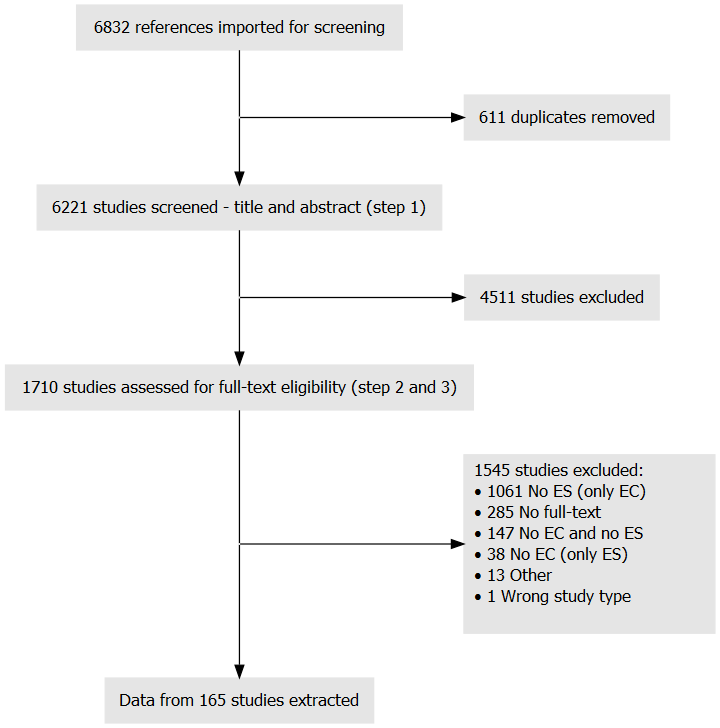
\includegraphics{figures/Pflow_chart.tiff}

}

\caption{\label{fig-figA1}PRISMA flow diagram for the evidence selection
process. ES signifies standards and EC signifies conceptualisations.}

\end{figure}%

The evidence selection process is also represented using the Preferred
Reporting Items for Systematic Reviews and Meta-Analyses (PRISMA) flow
diagram (Page et al., 2021) in Figure~\ref{fig-figA1}. Notably, two
rounds of exclusion occurred during the assessment for full-text
eligibility. 1710 studies entered step 2, 1223 were excluded and the
remaining 487 papers entered step 3. The data extraction template used
by the reviewers (authorship team) in step 3 revealed that, as expected,
inclusion was initially too generous, and some papers were not
sufficiently relevant, because of a lack of content on standards and/or
conceptual/theoretical elements. In this fashion, 322 papers were
further excluded and data extraction was completed to give a final
corpus of 165 papers. A summary of the reasons for exclusion of the 1545
papers (between steps 2 and 3) are included in Figure~\ref{fig-figA1}.

\begin{figure}

\centering{

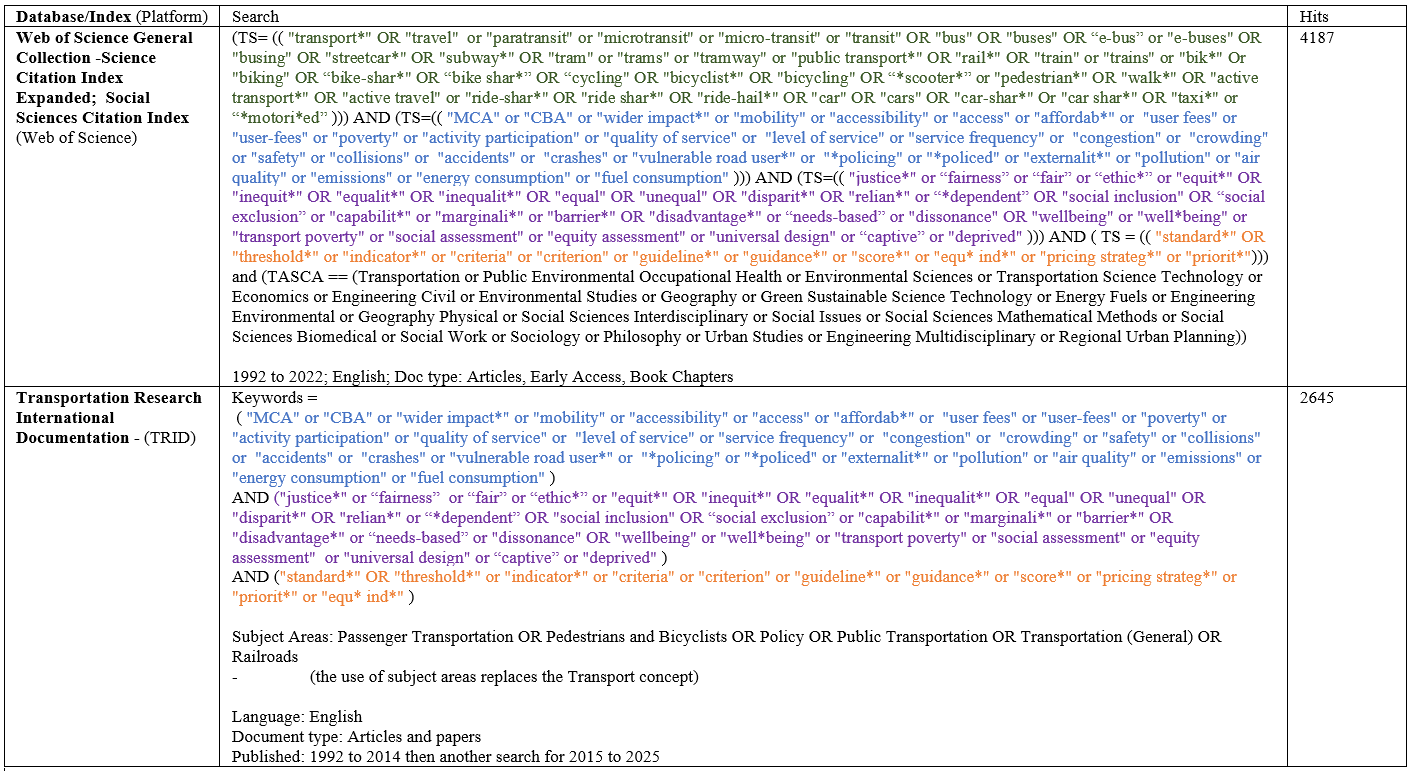
\includegraphics{figures/Search-query.png}

}

\caption{\label{fig-figA2}The search query. TS = topic search (keywords,
abstract, title). TASCA = subject categories. Green text area
transportation system related terms, blue text are equity dimension
related terms, purple text are equity/justice conceptualization related
terms, and orange text are standards related terms. Hits corresponds the
number of papers that the search yielded and was retained into the
evidence selection process.}

\end{figure}%

Definitions of the population-concept context (PCC) used in the creation
of the inclusion and exclusion criteria for the search strategy.

\begin{itemize}
\tightlist
\item
  \textbf{Population}: the focus of the included studies should be on
  individuals, groups, communities, or entire regional areas that are
  impacted by passenger transportation infrastructure and systems (i.e.,
  all modes and flows) from the perspective of equity (i.e., fair
  distribution, production, and re-production of burdens and benefits).
  This criteria is reflected in the creation of the first set of topic
  search terms that relate to transportation modes (e.g., ``walking'' OR
  ``cycling'' OR ``transit'' - see green text in Figure~\ref{fig-figA2}
  for the full list).
\item
  \textbf{Concept}: the included studies should also include equity
  dimensions and conceptualizes equity as discussed in the previous
  section. This inclusion criteria is reflected in the second and third
  set of topic search terms developed in the search strategy. These
  terms relate to types of equity dimensions (e.g., ``accessibility'' OR
  ``mobility'' or ``transport-related air pollution'' - see blue text in
  the Figure~\ref{fig-figA2} for the full list) and fairness
  conceptualizations (e.g., ``Justice'' OR ``equity'' - see purple text
  in Figure~\ref{fig-figA2} for the full list).
\item
  \textbf{Context}: the included studies should also be limited to
  publications that include types of standards. Context can be more
  difficult to explicitly search for with key terms so synonyms for
  `standards' were added to the query as a four set of topic search
  terms (e.g., threshold, indicator, criteria - see orange text in
  Figure~\ref{fig-figA2} for full list). Additionally, journal article
  and conference papers, English-language literature from any country,
  any study design (e.g., quantitative, qualitative, or mixed-method
  studies, or conceptual frameworks), and any record published within
  the past 30 years are included (January 1992 to March 2022). The time
  period is selected as the first (to the authors knowledge)
  peer-reviewed article which operationalized standards and fairness
  conceptualization was published in 1996 (Khisty, 1996); we are
  broadening the search by a few years for completeness. English is
  selected as it is the common language spoken across the authorship
  team. Furthermore, papers that explicitly fall within the
  Transportation or related topic/category is included in the query
  (e.g., ``Transportation'', ``Social Sciences'', ``Geography'', ``Civil
  Engineering'', ``Philosophy'' - see the Figure~\ref{fig-figA2} for
  full query).
\end{itemize}

The \textbf{exclusion criteria} for the search are papers that are not
within the inclusion criteria. Specifically:

\begin{itemize}
\tightlist
\item
  Literature published before January 1992.
\item
  Papers which do not include transportation equity dimensions.
\item
  Grey literature, as concepts contained within are frequently published
  in a more developed form in journals.
\end{itemize}

\subsection{Evidence selection and data extraction}\label{sec-sect62}

\begin{figure}

\centering{

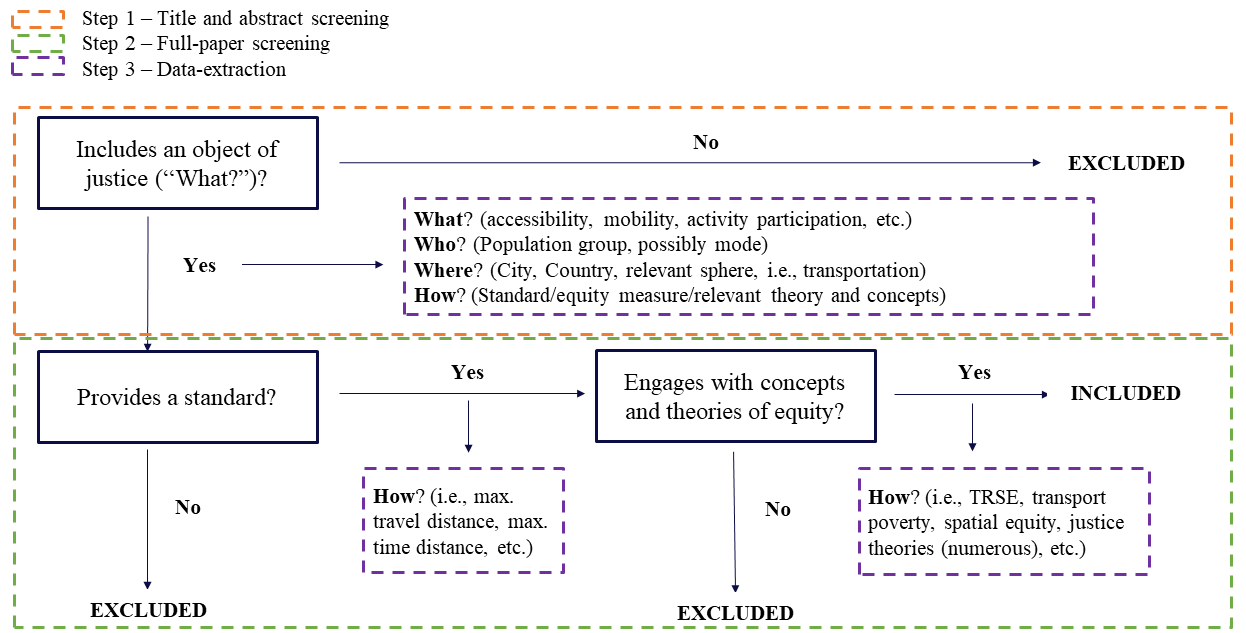
\includegraphics{figures/Methods_framework.png}

}

\caption{\label{fig-figA3}Evidence selection workflow. Step 1 (orange)
is title and abstract screening, step 2 (green) is full-text review, and
step 3 (purple) is data extraction.}

\end{figure}%

The following steps summarise the evidence selection process:

\begin{enumerate}
\def\labelenumi{\arabic{enumi}.}
\item
  The first step (orange box in Figure~\ref{fig-figA3}) included
  screening all titles and abstracts of papers on whether they included
  transportation equity as defined by the PCC. Each paper was screened
  by two independent reviewers who then voted for inclusion, exclusion,
  or uncertain inclusion. All uncertain papers, conflicting papers, and
  papers missing abstracts were reviewed by a third person for inclusion
  or exclusion.
\item
  The second step (green box in Figure~\ref{fig-figA3}) included
  scanning all full-text papers which passed step 1. These papers were
  reviewed to determine if they included a relevant ``how'', i.e., an
  standard and/or relevant theoretical or conceptual discussion. At this
  stage, papers were evaluated again by two independent reviewers who
  voted for inclusion or exclusion. If an article was voted to be
  excluded, it was tagged with one of five possible reasons for
  exclusion, namely (1) no standards included; (2) no relevant
  conceptual elements included; (3) no standard and no conceptual
  elements included; (4) send back -- QA issue; or (5) other.
  Discrepancies were resolved by a third reviewer.
\item
  In the last step, a data extraction template for each record was
  filled by one reviewer (purple box in Figure~\ref{fig-figA3}). The
  data extraction template was created with the aim of striking a
  balance between the complexity of categories and the simplicity of
  summary; information related to ``Where?'' (the geographical context
  and sphere of life), ``When?'' (temporal circumstances for the
  application of justice), ``Who?'' (the subject of justice), ``What?''
  (the object of justice), and ``How?'' ( standards and
  conceptualisations) was filled out for each study. The following table
  contains the template that was input into \emph{Covidence} and used
  throughout.
\end{enumerate}

Data extraction for each document that passed through all three steps
was then extracted using this template:

\begin{figure}

\centering{

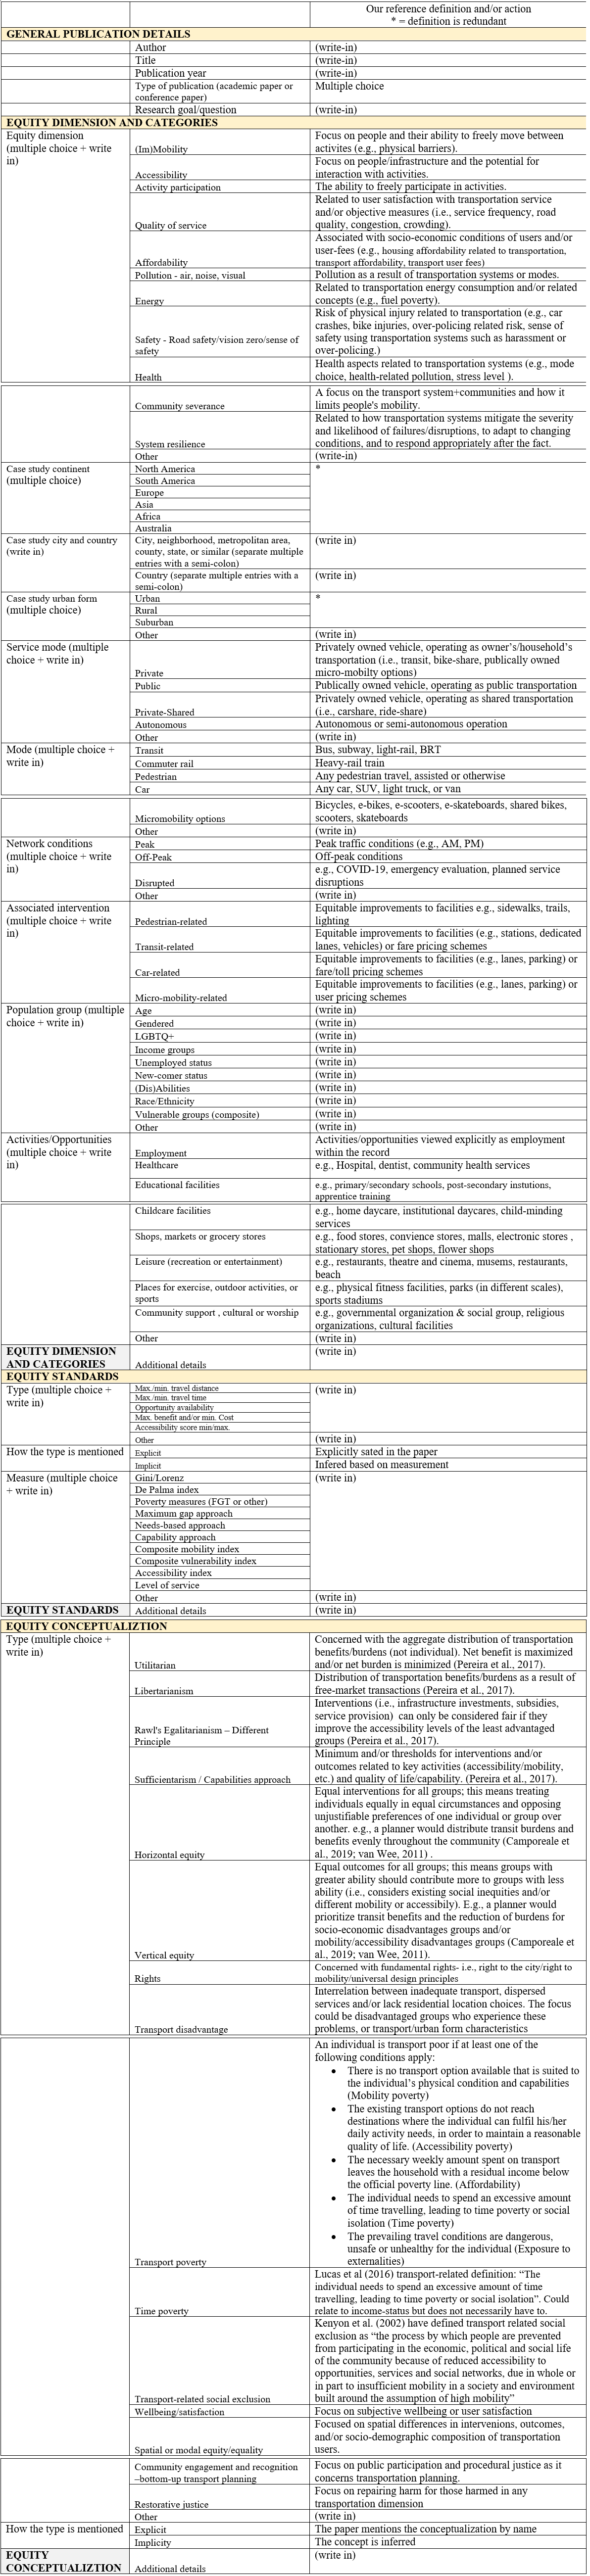
\includegraphics{figures/Data-extract-template.png}

}

\caption{\label{fig-figA4}The data extraction template with associated
defintions.}

\end{figure}%

\subsection{Select reviewed works summarized by the
5WH}\label{sec-sect63}

\begin{table}
\begin{tabular*}{\linewidth}{@{\extracolsep{\fill}}llll}
\toprule
Dimension & Continent & Conceptualization & Standard \\ 
\midrule\addlinespace[2.5pt]
What?: **mobility and accessibilty** & Where? [@rivasHowAffordableTransportation2018] - South America (select cities) & Analyses how affordable urban public transportation is in select Latin American and Caribbean countries. They look at the estimated average monthly cost of transit trips and average monthly household income and conceptualize **transport-related** **affordability**, especially for the most economically vulnerable (**vertical equity**). & How?: The financial burden of a basket of urban public transportation trips (60 trip fares, representing 30 round-trips per month) should not exceed 10\% of household monthly income. \\ 
What?: **mobility and accessibilty** & Where?: [@bharathyRevisitingClearFloor2018] - North America (USA - National) & This study designed a web-based tool and took a representative sample of wheeled mobility device (WhMD) users anthropometry measurements to determine if the minimum standard suggested by the ADA is sufficient. We understand this conceptualization as a type of **Rights** conceptualization that WhMD should have minimum clear floor space (as described the guidelines in line with the American Disabilities Act) to access bus shelters, bus stop pads, and transit terminals. & How?: The clear floor area for wheelchairs: 760 mm (30 in.) wide by 1220 mm (48 in.) in length as described by the ADA standards. Of note, this minimum clear floor area is insufficient for a variety of the WhMD users. \\ 
What?: **mobility and accessibilty** & [@ryanWhatAreWe2021] - Europe (Stockholm, Gothenburg and Malmo cities in Sweden) & Investigates what the literature and planning process is missing when we measure accessibility by comparing objective and self-reported accounts of accessibility among older people. This paper conceptualizes accessibility as from the position of the **capabilities approach** and **vertical equity** (particularly acknowledging that older people have capabilities that differ from the general population). & How?: Specifically for older populations (aged 65+), the following travel distances are suggested as equitable trip lengths to grocery stores per mode: Walking: less than or equal to 1500m, Combined transit and walking (less than or equal to 1000m (walking element)), Combined car and walking: less than or equal to 1000m less than or equal to 1000m (walking element)), Bicycle: less than or equal to 3000m in addition to travel time threshold of less than 15 mins. \\ 
What?: **mobility and accessibilty** & Where?: [@wismadiSpatialPreferenceModelling2014] - Asia (Yogyakarta, Indonesia) & Explores the equitable provision of transport infrastructure provision: an application of Sen's **capability approach**. Conceptualizes equity through Sen's capability approach and spatial equity. & How?: Areas below the relative poverty line (of its neighbours) can only be located transport resources (i.e., measure in person*kms that can be travelled at car speed, i.e., mobility) based on the following 2 benchmarks (they can be considered, together as the floor/minmum access): 1) Global: standard deviation (SD) distance to mean should be minimized. 2) Local: priority to minimise the differences with its neighbourhood \\ 
What?: **mobility and accessibilty** & Where?: [@zhengAreabasedEquitablePricing2020] - North America & This paper conceptualizies equity in the multimodal network (transit, car) being fair toll-pricing across differences in populatins value of time (VOT). VOT is determined based on household income, with lower income households having lower VOT and thus deserving of lower tolls (vertical equity). From this perspective, a utilitarian perspective that seeks to minimize multimodal traffic congestion through introducing toll-pricing based on VOT is implemented. & How?: suggest that a toll-pricing scheme based on individuals travel value-of-time (lower income people have a lower VOT) is equitable. \\ 
What?: **environmental pollution** & Where?: [@carrierApplicationThreeMethods2014] - North America (Montreal, Canada)  & This work examines the statistical association between different social groups and the concentration of air pollutants. They frame their work from the perspective of environmental equity. We interpret the conceptualizations to be along the lines of **inequitable externalities**, **spatial** and **vertical equity** - transport-related air pollution is a product of road transport and it impacts the air of residents in unequal spatial ways. The paper then frames this impact as unfair, particularly from the perspective of disproportionately disadvantaged residents & How?: The literature suggests that the health implications from the transport-related air pollution from major roadways is most acute at residential distance locations of 200 m or less. Residential locations should not be located within this distance threshold from the perspective of human health. **Environmental+** and **Population standards**: Uses the WHO NO² threshold as a point of comparison (annual concentrations of NO² should not exceed 40 μg/m-3). They argue that even through no neighbourhood, even those disproportionately low income, exceed the WHO limit in this case study, they still suggest that air pollution should not be disproportionately impacting disadvantaged neighbourhoods. It can be interpreted that they use the WHO threshold as a minimum threshold and suggest that air pollution levels should not be impacting disadvantaged populations disproportionately ( a relative population standard) \\ 
What?: **environmental pollution** & Where?: [@jephcoteGeospatialAnalysisNaturally2013] - Europe (Leicester, UK) & Geospatial analysis of naturally occurring boundaries in road-transport emissions and childrens respiratory health across a demographically diverse cityscape. Emperically identifies at what distance away from major roadways children are most impacted by transport-related pollution. This is framed in the perspective of children’s **well-being**. Children are at most risk for acute respiratory distress from elevated levels of air pollution, and as such planning should consider this point of public health. & How?: Finds that children (most vulnerable to air pollution - related to motoized traffic) are most impacted by air pollution within 283 m of a road way. This should be the distance threshold that schools and other childrens facilities are located. \\ 
What?: **health impacts** & Where? [@adlakhaMindGapGender2020] - Asia (Chennai, India) & From the perspective of disparity in gendered physical activity, this paper focuses on women's cycling as both transport and exercise. They advocate for all people achieving physical activity thresholds (**horizontal equity**) but prioritize women and especially women in neighbourhoods with low-walkability and socio-economic status (**vertical equity**). & How?: All people should get 150 min of moderate activity a week or 75 min of vigorous physical activity per week. \\ 
What?: **health impacts** & Where? [@savingmothersDidSavingMothers2019] - Africa (Select urban and rural regions in Uganda) & The **well-being** of mothers, this paper examines the timely access to emergency obsteric and newborn care for child-bearing aged women in Uganda. & How?: 2 hours to the nearest facility with surgical capacity with anesthesia services - this threshold is determined through the onset of bleeding to death if a women with obstetric hemorrhage does not receive adequate treatment). \\ 
What?: **health impacts** & Where?: [@iungmanImpactUrbanTransport2021] - Europe (Madrid and Barcelona, Spain) & They use environmental pollution guidelines, but from the position of health. They investigate the impact of urban and transport planning on attributable mortality burden in Madrid and Barcelona and its distribution by socioeconomic status . Pre-mature mortality is linked to the exposure to pollution and motorized vehicles (**inequitable externalities**). These externalities should not be impacting people disproportionately (**vertical equity**) and should be even across space (**spatial equity**). & How?: All minimum thresholds, if exceeded this is inequitable: NO² concentration 40 μg/m³; PM 2.5 concentration 10 μg/m³; Noise 53dB for average 24 hours; Living with 300 m crow-flies distance from at least .5 hectares of greenspace; and a Change of air temperature of at least 1 ⁰C.  \\ 
What?: **health impacts** & Where?: [@mehdizadehWalkingTimeSchool2017] - Asia (Rasht, Iran) & From the perspective of children’s **well-being**, assesses the walking time to school. They frame walking to school as health-related. & How?: perceived walking time to school for students aged 7-9 yrs is 10 mins, and the longer the PWTS the less likely they were to use an active mode to travel to school. \\ 
What?: **health impacts** & Where? [@murphySupermarketAccessTransport2017] - Oceania (Melbourne, Australia) & Assesses the relationship between supermarket access and transport mode used, the body mass index (BMI) of the mode-user (**wellbeing**) and the equity in access distribution by income (**vertical equity**). & How?: all households should be sufficiently active (greater than 150 min and at least 5 sessions) and households should be within 1 km euclidean distance to supermarket (80-90\% of the dwellings should meet this). Planners should prioritize socially disadvantaged areas to meeting these standards first. \\ 
What?: **transport-related safety** & Where?: [@ferenchakEquityAnalysisProactively2019] - North America (Denver, USA) & Operationalizes and compares an equity analysis of proactively- and reactively-identified traffic safety issues from the perspective of **Spatial equity**, **Vertical equity** and **Inequitable exposure to externalities**. & How?: standards are suggested for both reactive and proactive analysis. First, the lower the number of collisions on the road with pedestrians/cyclists (i.e., reactive safety analysis), the better. No/minimal inequalities for general population vs. equity seeking groups (high proportion of POC and/or low income in tract). Second, the lower the perceived safety, the better (i.e., if travel to school by ped. or bike is unsafe due to traffic conditions). No/minimal inequalities for general population vs. equity seeking groups (high proportion of POC and/or low income in tract). \\ 
What?: **transport-related safety** & Where?: [@zheEvaluationSharedUse2008] - Asia (Tokyo, Takamatsu, and Tokushima) & Evaluates the observed safety of  shared use pedestrian and bicycle paths from the perspective of **well-being**. & How?: the study suggests that the safety threshold for bicycles and pedestrians to coexist on shared infrastructure is less than 0.5 pedestrians/minute per metre of sidewalk (width) and less than 3.0 cyclists/minute per metre of sidewalk (width). The standard for pedestrian/bicycle share use in terms of hourly traffic volume is less than 26 pedestrians / hour and 108 cyclists / hour for 2m wide sidewalks. \\ 
What?: **mobility/accessibility and health impacts** & Where?: [@aldertonWhatMeaningUrban2019] - Asia (Bangkok, Thailand) – **Mobility/ accessibility** and **health** & Establishes short-, medium-, and long-term goals for the city in collaboration with technical leaders within the municipal government for the perspective of **well-being** (urban livability): the standards included in this table relate directly to transportation systems. Indicators are inspired by the Sustainable Development Goals (SDGs) as well other global planning standards. & How?: 1) Green space: \% of residents living < 400 m from public open space, a large park (> 1.5ha), and/or local park, 2) transit access: \% of residents living < 400 m of a local bus stop and <800 m of train station, 3) Facilities: \% of residents living < 400 m of a community centre. The following **Infrastructure standard** is suggested: Canal water quality - dissolved oxygen content of equal to or less than 2.0 mL/L \\ 
What?: **Mobility/ accessibility** and **health impacts** & Where?: [@berheAdaptationDissonanceQuality2014] - Africa (Mekelle, Ethiopia) & Examines adaption and dissonance in the quality of life (QoL) of residents. QoL is conceptualized along the lines of **well-being** and aspects of QoL directly tie into transport systems. They conduct a qualitative QoL survey of residents on the topic of three QoL domains: housing quality, access to important destinations, and affordability. They also measure quantitative indicators associated with these domains. We assume the equity goal for this paper is that subjective and objective QoL measures should not be mismatched: as discussed by the authors of this study, subjective QoL is higher than objective QoL the participant is experiencing adaption and in the reverse scenario the participant is experience dissonance. & How: 1 \& 2) Access to primary or secondary education facility, percentage of households living within 1 km or 2km (walking distance), respectively from a primary school or secondary school. 3) Access to health facility, percentage of households within 40 min walking time from a health facility. 4) Access to public transport, percentage of households within a distance of 500 m from a mini-bus stop. **Population standards**: 1) Adequate family income, percentage of households earning more than the official poverty line. 2) Subjective QoL is constructed based on the households level of satisfaction for each of the eight indicators using a six point Likert-scale (1=very satisfied to 6=very dissatisfied). \\ 
What?: **mobility/accessibility, health impacts, and safety** & Where? [@agostfelipInclusiveModelAssessing2021] - Europe (Castellon, Spain) & Conceptualizes equity through age-friendly urban spaces that reduce (and eliminate) conditions for **transport-related social exclusion** for older populations and prioritize those who are economically vulnerable (**vertical equity**). These guidelines are inspired by the SDGs in addition to planning guidelines used national, regional, and local guidelines used in Spain. & How: 1) Access to facilities needed for old age health. Minimum distance thresholds from the geometric center of neighbourhood are suggested: at least: 1000 m from health facilities (600 m or less is preferred), elderly-specific care facilities and shops should be 600 m (300 m or less is preferred). **Population standards**: 1) Certain neighbourhoods should be prioritized above others. From this papers focus on age-friendly urban environment, they suggest that if the neighbourhood has an average old age indicator (i.e., greater than 64 years, and/or greater than 79 years, and/or aging ratio of persons aged greater than 64 relative to 15 to 64 age) should be prioritized. 2) Economic vulnerable and non-civically engaged neighbourhoods should also be prioritized. If the neighbourhood has a lower percentage of civic associations within the neighbourhood than average, and/or household income, and/or a higher than average interventions for dependency and/or social subsidies, they should be priorized. **Infrastructure standards **: 1) Green space: should be at least 10 m2 per inhabitant in the neighbourhood, greater than 15 m2 per inhab. is the goal. 2) As related to sidewalk infrastructure at least 50\% of all sidewalks (preferably 75\% or greater) should: have a width of 1.5m or larger, ramps should have a grade of 8\% or less, be well maintained (free from deficiencies), be paved for pedestrian use, and cover transit stops. 3) Lighting is critical for traffic-safety and a sense of safety overall. As such, at least 50\% roads should: have a min. of 35 lux (road traffic) and 20 lux (pedestrian streets), and adapted traffic lights. 4) Buildings should be age-friendly. As a proxy for the quality of residential living space quality, at least 50\% of residential buildings in a neighbourhood should be built within the last 50 years (preferably 75\% or more). In terms of physical access into the buildings, at least 10\% should have elevators and accessible entrances (preferably 25\% or more). **Environment + standards **: 1) Noise at the street level should be less than 55 dB and 45 dB (but preferably less than 50 dB and 40 dB) in the daytime and nighttime, respectively. \\ 
What?: **mobility/accessibility and safety** & Where?: [@mateobabianoPedestrianNeedsMatter2016] - Asian (Manila, Philippine) & The perception of pedestrians’ walking environments should be sufficient across 6 themes. Equity is conceptualized around **spatial equity** (equally fair walking environments for all locations) and **rights** (the right to mobility/accessibility for pedestrians) & How?: perceived pedestrian perception on protection, ease, equitable access, mobility, identity, and enjoyment must be met. \\ 
\bottomrule
\end{tabular*}
\end{table}



\end{document}
